\documentclass[twoside,project]{../MFFPrace}

\usepackage{subfigure}
\usepackage[backend=biber,style=numeric,sorting=none]{biblatex}
\usepackage{changepage}

\NazevPrace{Chromatická holografie}
\AutorPrace{Bc.~Michal~Ciesla}
\RokOdevzdani{2023}
\Katedra{Katedra chemické fyziky a optiky}
\Vedouci{RNDr.~Eva~Schmoranzerová,~PhD.}
\Konzultant{Mgr.~Zeynab~Sadeghi}

\addbibresource{reference.bib}

\begin{document}
\maketitle
\tableofcontents
\chapter*{Úvod}
\addcontentsline{toc}{chapter}{Úvod}
\textit{Holografie} je metodou zachycení a reprodukce obrazu, která narozdíl od \textit{fotografie} nezachycuje výsledný dvourozměrný obraz, nýbrž původní předmětovou vlnu světla. Díky tomu umožňují hologramy reprodukovat zaznamenaný objekt v jeho trojrozměrné podobě, tj. lze objekt pozorovat z více úhlů tak, jako by se objekt na daném místě skutečně nacházel.

Hologramy je možné vytvářet ve dvou variantách: \textit{reflexní} a \textit{transmisní}. Reflexní hologramy jsou jednodušší jak na výrobu, tak na pozorování -- na expozici je potřeba pouze jeden svazek koherentního světla a pozorovatelné jsou i v běžném bílém světle -- vytvářejí ovšem pouze virtuální obraz. Hologramy transmisní vyžadují rozdělení svazku na alespoň dvě větve ve vhodném poměru a zobrazovat je lze pouze koherentním světlem stejné vlnové délky, ovšem vytvářejí virtuální obrazy i reálný obraz, který lze promítat na stínítko. Tento reálný obraz navíc lze dále použít pro proces tzv. \textit{sekundární holografie}, díky kterému lze existující hologramy kopírovat.

Cílem tohoto projektu bylo sestavit, resp. aktualizovat, experimentální uspořádání pro záznam a zobrazování hologramů, a to hologramů plně barevných. Toto vyžaduje zapojení tří laserů (červeného, zeleného a modrého) do experimentálního uspořádání a jejich současnému navedení na plochu holografické desky. Při tomto procesu jsme se setkali s řadou kuriozit a komplikací, které popisuje první kapitola.

\chapter{Výchozí stav a experimenty}
\begin{center}
    Na začátku úlohy jsme vycházeli z existujícího experimentálního uspořádání pro holografii. To bylo sestaveno pro holografii monochromatickou, a to vzhledem k velmi úzké spektrální citlivosti dříve používaných holografických desek. Toto existující uspořádání jsme využili pro vyzkoušení procesu s původními deskami a ověření fungování nových holografických desek.
\end{center}
\section{Původní uspořádání}
Existující uspořádání bylo uzpůsobeno pro monochromatické hologramy zelené barvy o vlnové délce $532\,\text{nm}$, na kterou jedinou byly citlivé používané chemické holografické desky. Proces vyvolávání těchto desek vyžadoval práci s nebezpečnými chemikáliemi, časově náročnou přípravu a proces vyvolávání, též časově náročný a obnášející vkládání desek do chemických roztoků, musel probíhat za velmi slabého osvětlení červeným světlem. Chemikálie i holografické desky samotné rychle degradovaly a často se díky tomu hologramy nepodařilo vytvořit vůbec. Tyto faktory byly tlakem ke změně.

\begin{figure}
    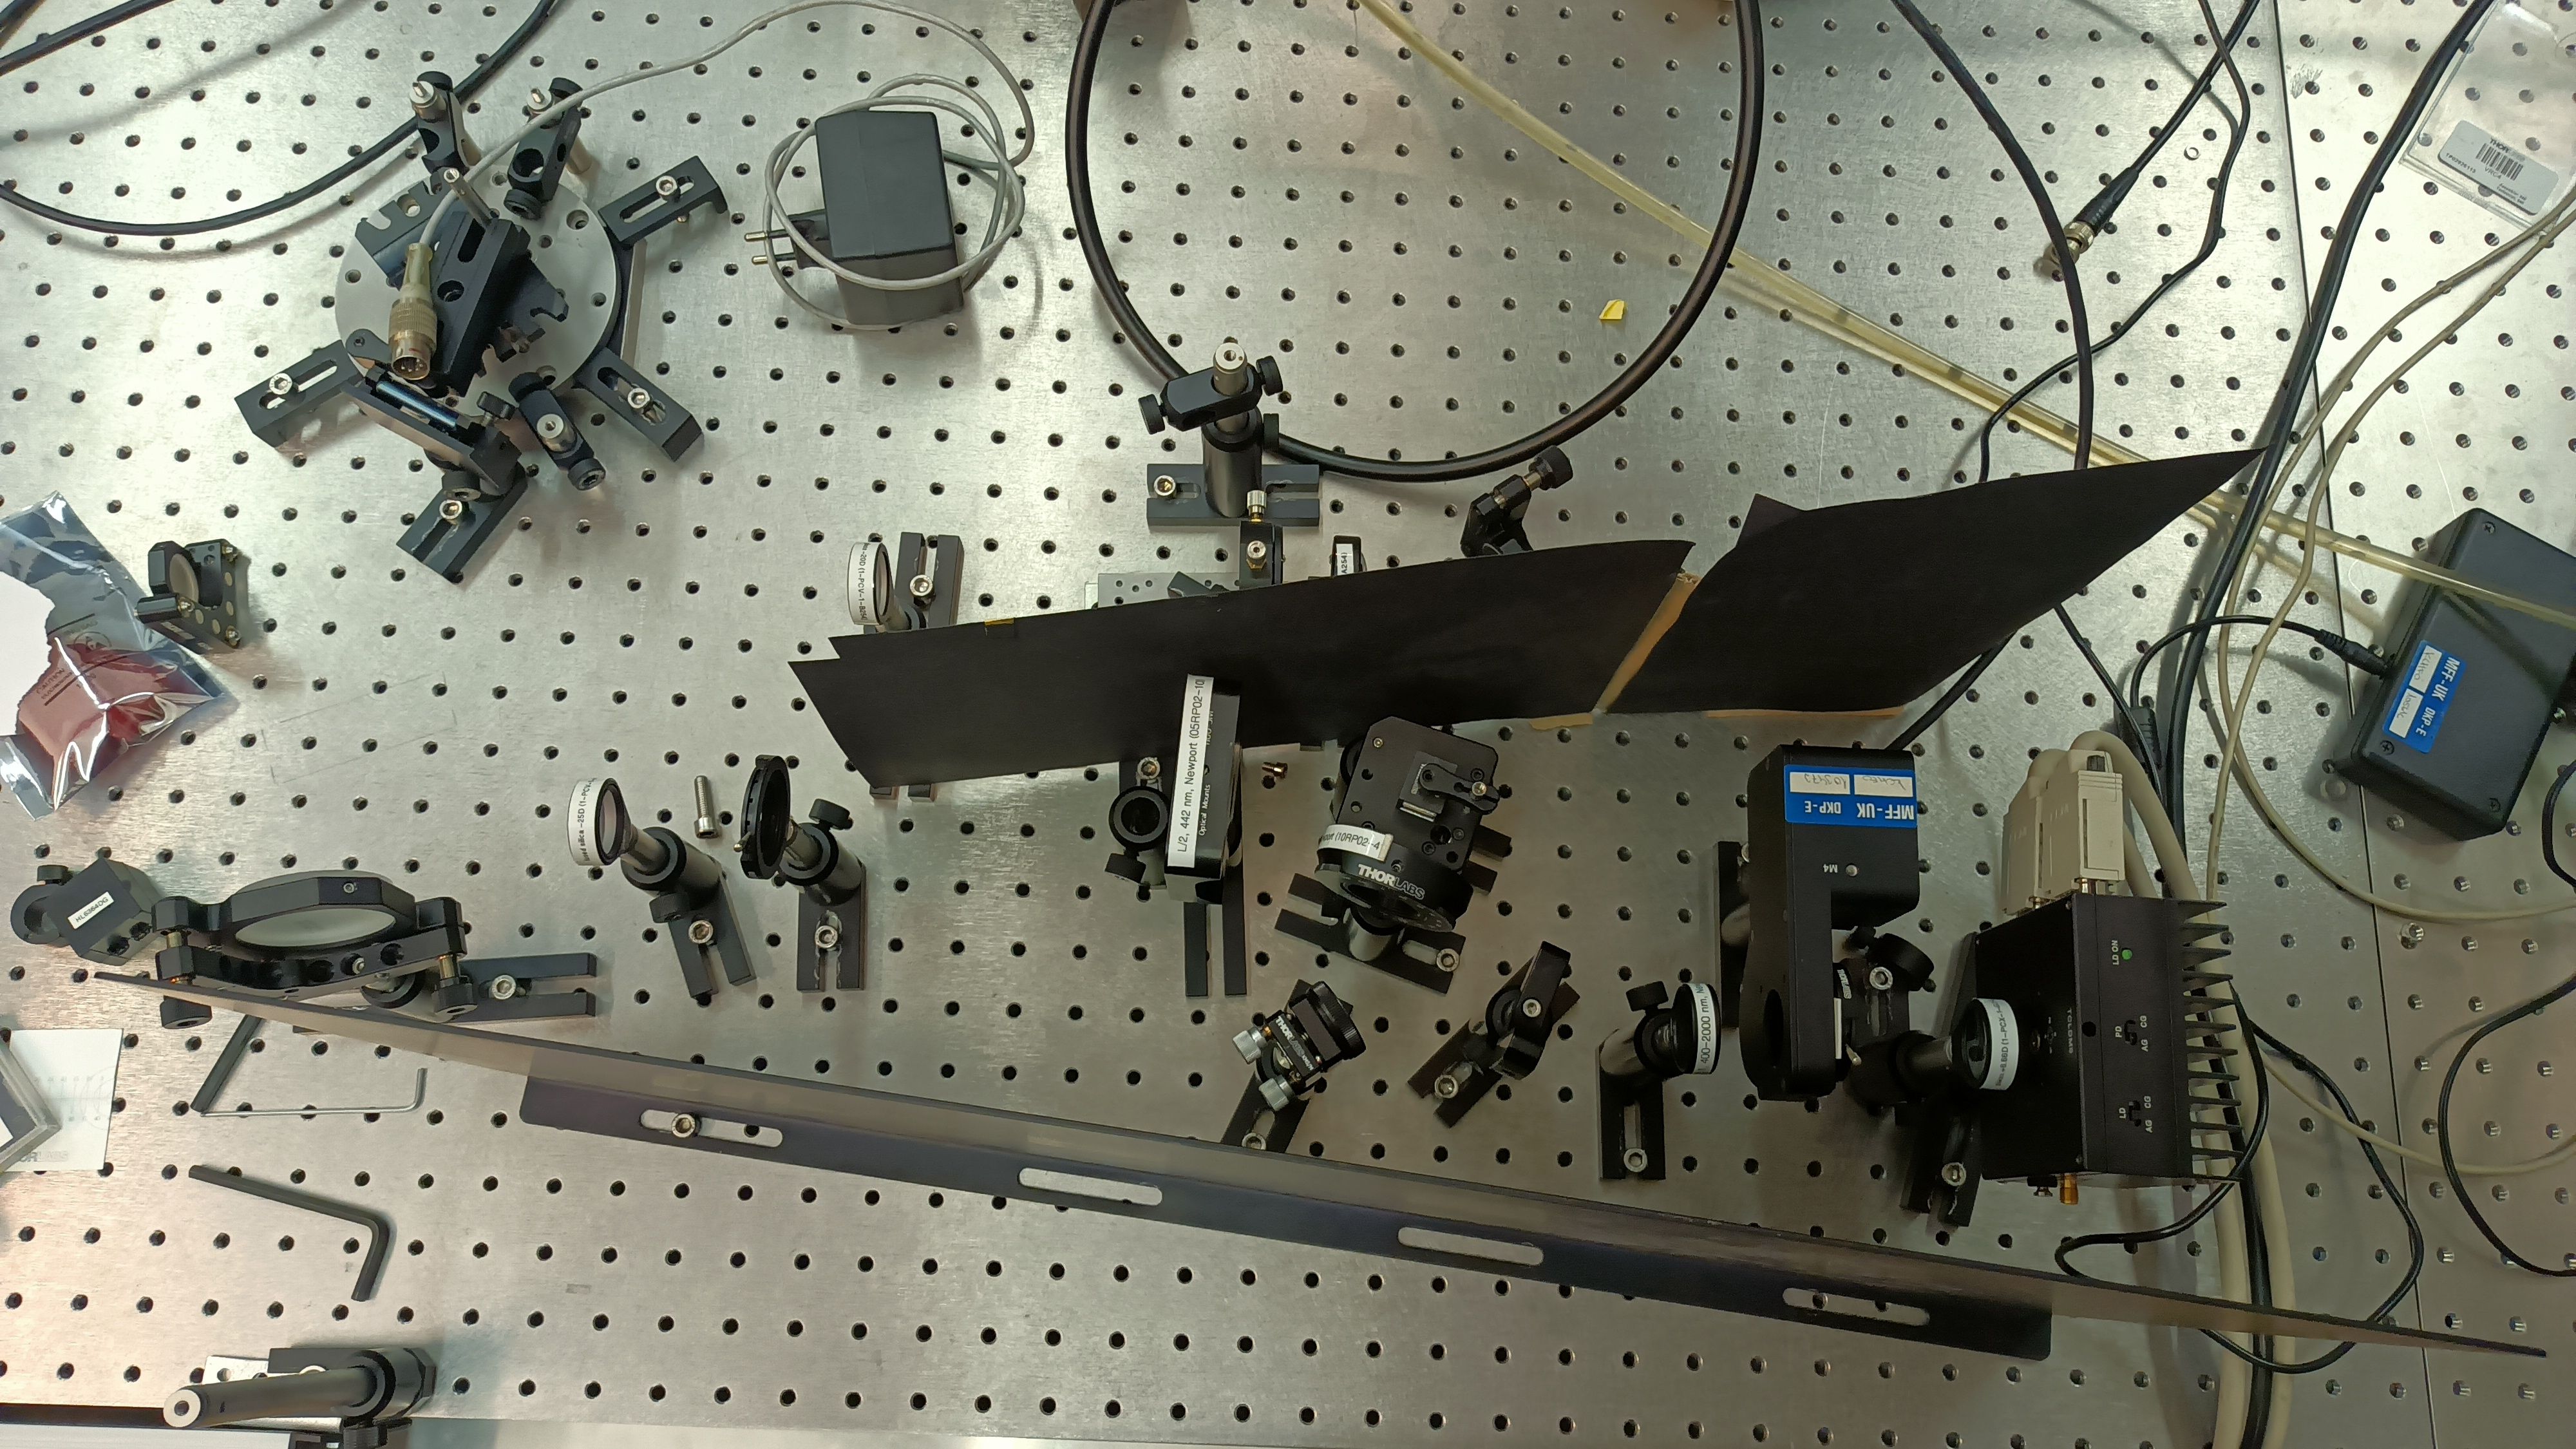
\includegraphics[width=\linewidth]{../img/stare-usporadani.jpg}
    \caption{Původní experimentální uspořádání}
    \label{img:puvodni-usporadani}
\end{figure}

Obrázek \ref{img:puvodni-usporadani} ukazuje původní experimentální uspořádání holografie. Laserový paprsek vychází zprava, je kolimován spojnou čočkou a prochází elektronicky otevíratelnou clonou, která sloužila k ukončení expozice po potřebném čase. Dále paprsek prochází šedým filtrem, který dodatečně snižuje jeho intenzitu, a po odrazu na zrcátku prochází půlvlnovou destičkou, která určuje jeho polarizaci. Dále svazek světla vstupuje do polarizačního děliče, který v kombinaci s předešlou půlvlnovou destičkou umožňuje rozdělení svazku do dvou ramen s nastavitelným poměrem intenzit pro účely transmisní holografie. Jedno z ramen pokračuje doleva, prochází další půlvlnovou destičkou a po průchodu irisovou clonkou, která odstiňuje nežádoucí odrazy, je zvětšeno rozptylnou čočkou a odraženo na holografickou desku a objekt v levém horním rohu. Toto rameno slouží reflexní holografii i jako referenční vlna v transmisní holografii. Druhé rameno polarizačním děličem pokračuje rovně na obdobnou zvětšující soustavu, která je na fotografii zakryta papírovým stínítkem, a slouží pak jako objektová vlna v transmisní holografii.

\medskip

V rámci úvodních pokusů jsme se provedli dva pokusy o výrobu hologramu na chemických deskách, ani jeden z pokusů však nebyl úspěšný. V prvním případě došlo k přeexponování desky, v druhém případě se pravděpodobně vzhledem ke stáří chemikálií nepodařilo desku vyvolat.

V tomto uspořádání byly také provedeny pokusy na nových holografických deskách, které umožňují plně barevný zápis. Pokusné expozice byly monochromatické, jelikož toto uspořádání neumožňovalo navedení více laserových svazků naráz, nicméně tyto pokusy posloužily k určení vlivu kvality laserového svazku na výsledný hologram, který je popsán v sekci \ref{sec:diody}.


\section{Návrh nového uspořádání}
Důležitý požadavkem na nové uspořádání byla možnost jednoduchého přemístění. Z toho důvodu bylo celé nové uspořádání stavěno na desce velikosti $60\,\text{cm}\times30\,\text{cm}$, kterou je možné jednoduše zvednout a přemístit bez potřeby jakékoli demontáže. Pro barevnou holografii bylo také potřeba zajistit vstup tří laserových paprsků, plus bylo již od začátku počítáno s možností navedení čtvrtého, externího, laserového paprsku pro experimenty s lasery jinými, než jsou v uspořádání umístěné napevno.

\begin{figure}
    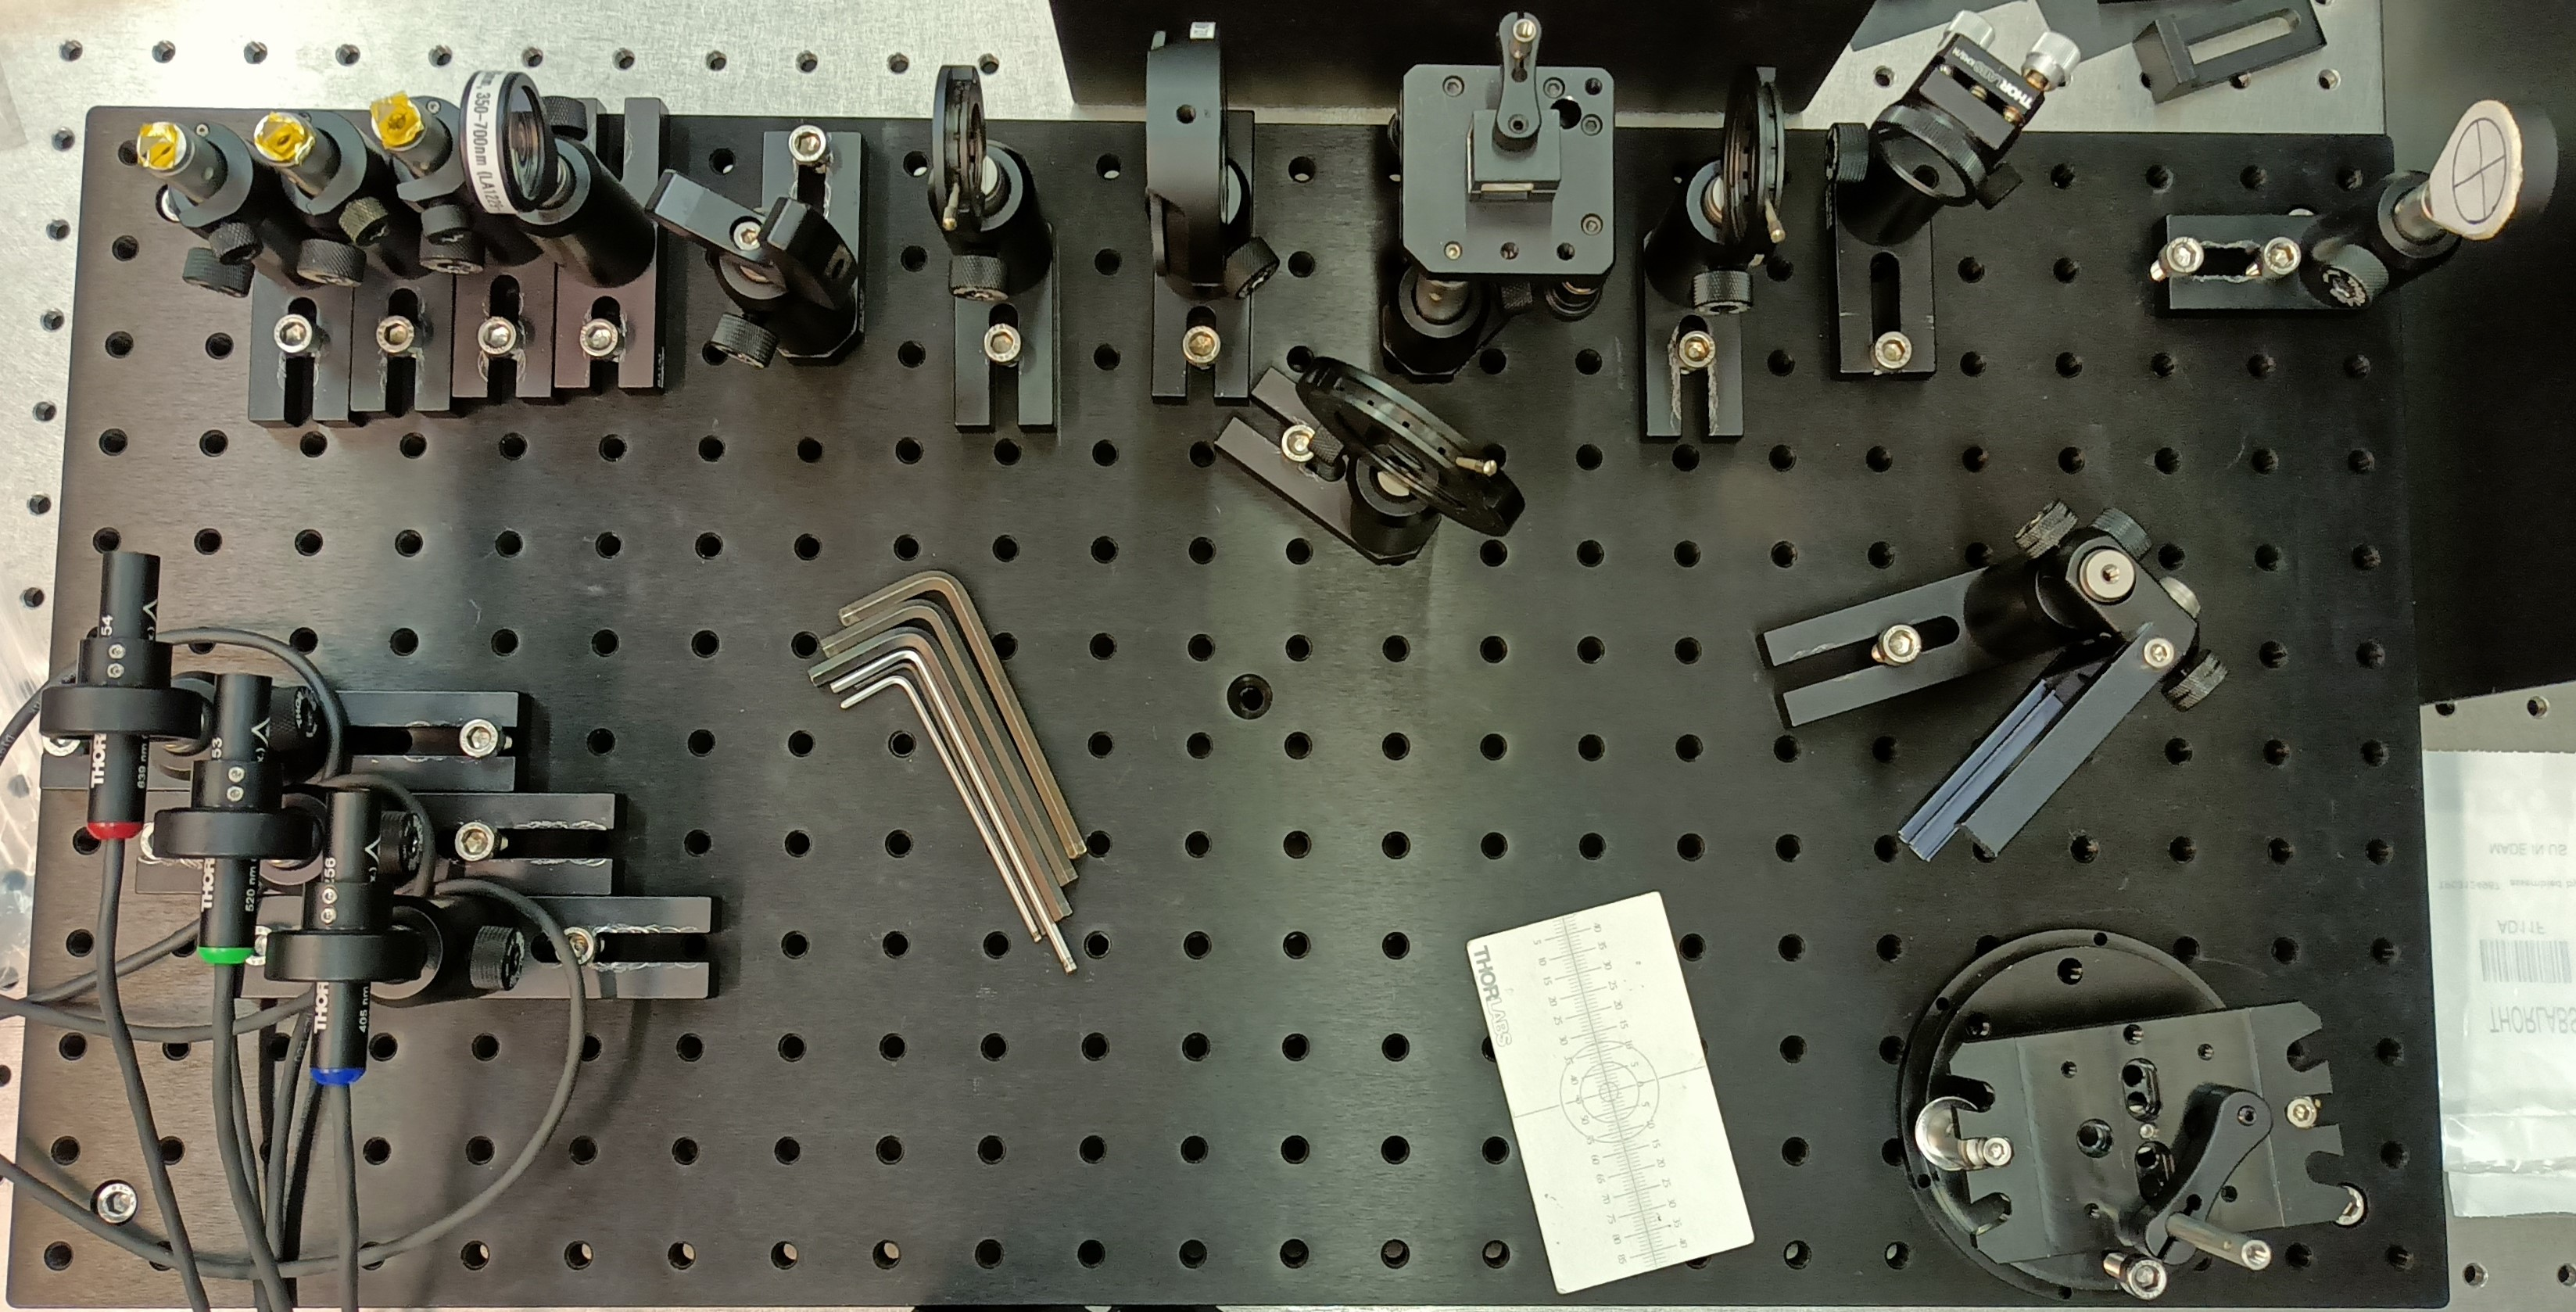
\includegraphics[width=\linewidth]{../img/nove-usporadani-prvni.jpg}
    \caption{První iterace nového experimentálního uspořádání}
    \label{img:prvni-iterace}
\end{figure}

První iterace pro účely testování konceptu je na obrázku \ref{img:prvni-iterace}. Paprsky z trojice laserových diod jsou odraženy malými zrcátky umístěnými tak, aby paprsky dále pokračovaly co nejblíže sobě. Dále procházejí spojnou čočkou pro kolimaci a irisovou clonkou pro kalibraci a odstínění divokých odrazů. Následně je použita stejná kombinace půlvlnové a polarizačního děliče jako v původním uspořádání pro rozdělení kombinovaného svazku na dvě ramena pro transmisní holografii. Rameno objektové vlny je na obrázku \ref{img:prvni-iterace} ukončeno další irisovou clonkou pro kalibraci a odstínění, druhé rameno je vedeno skrz irisovou clonku na rovinné zrcátko, které svazky směruje na držák holografické desky a podstavec pro objekt.

Chybějící v této iteraci byla rozptylná čočka pro rozšíření svazku dopadajícího na desku a objekt a celé rameno objektové vlny, které by se skládalo z hranolového děliče svazku a soustavy zrcátek a rozptylných čoček pro osvícení objektu ze dvou stran.

\medskip

Základní formát tohoto uspořádání byl zachován i do výsledného uspořádání (viz kapitola \ref{cpt:optika}). Vzhledem k problémům se svazky používaných laserů popisovaných dále v sekci \ref{sec:negauss} však musely být všechny čočky nahrazeny sférickými a/nebo parabolickými zrcátky, tedy se výsledné uspořádání zjednodušilo o veškeré čočky.


\section{Úskalí laserových diod\label{sec:diody}}
Při úvodních experimentech na starém uspořádání jsme nové desky testovali na třech různých laserových zdrojích.

Prvním byl zelený solid-state laser o velmi konstantní vlnové délce $532\,\text{nm}$, který byl používán i v původní úloze. Tento laser má velmi kvalitní tvar svazku, gaussovské rozložení intezity světla a světelný výkon $40\,\text{mW}$. Po zvětšení a expozici v reflexním uspořádání dával ze všech nejlepší výsledky -- poskytoval potřebné homogenní osvětlení desky; zvětšený svazek i výsledný hologram je na obrázku \ref{img:svazky-g}. % FIXME: Solid-state ???

\begin{figure}[!ht]
    \centering
    \subfigure[solid-state]{ % FIXME: Solid-State ???
        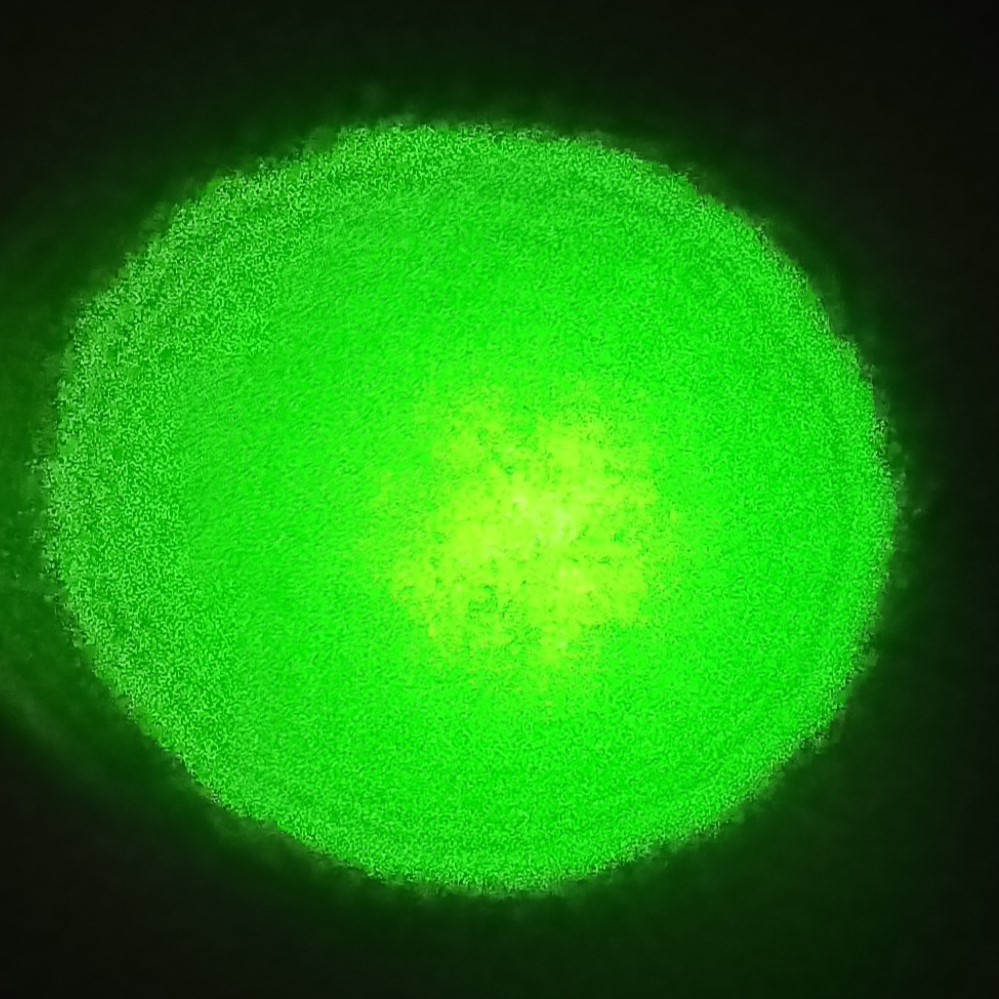
\includegraphics[width=0.3\linewidth]{../img/svazek-g.jpg}
        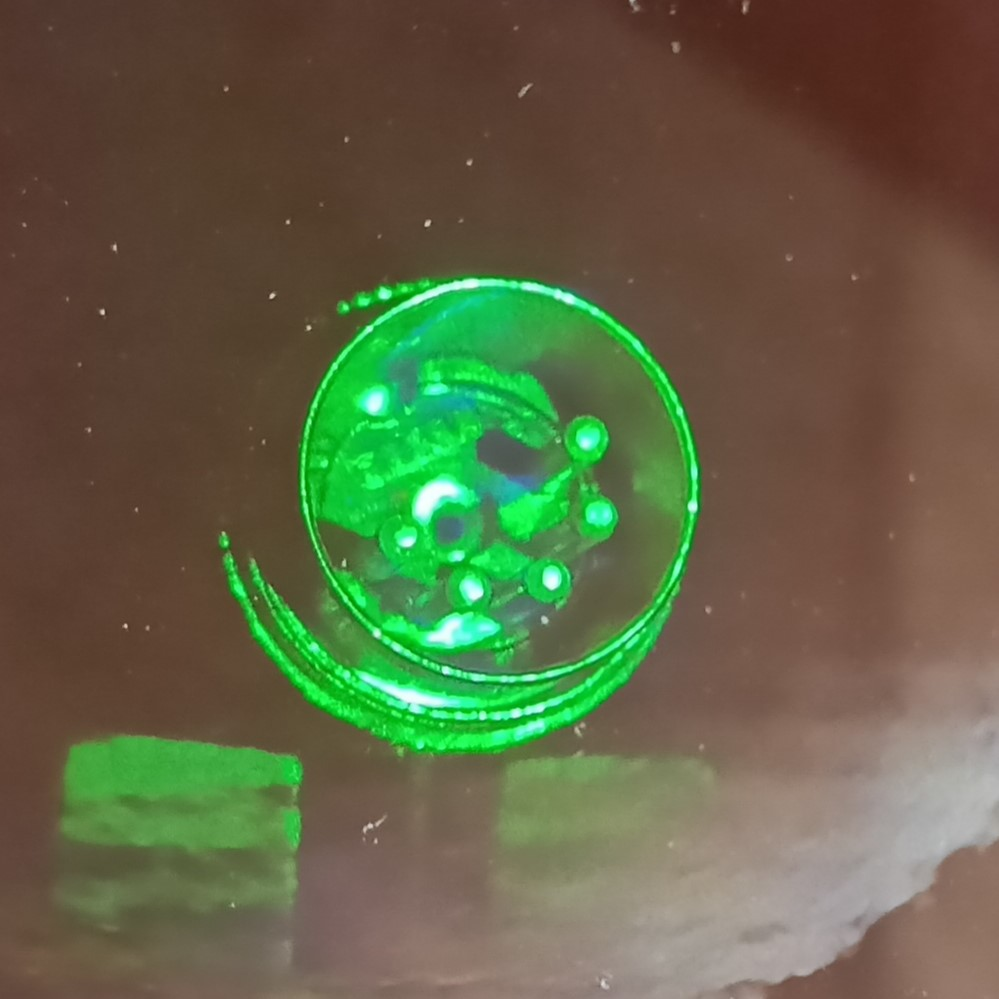
\includegraphics[width=0.3\linewidth]{../img/hologram-r-g.jpg}
        \label{img:svazky-g}
    }
    \subfigure[alignment]{
        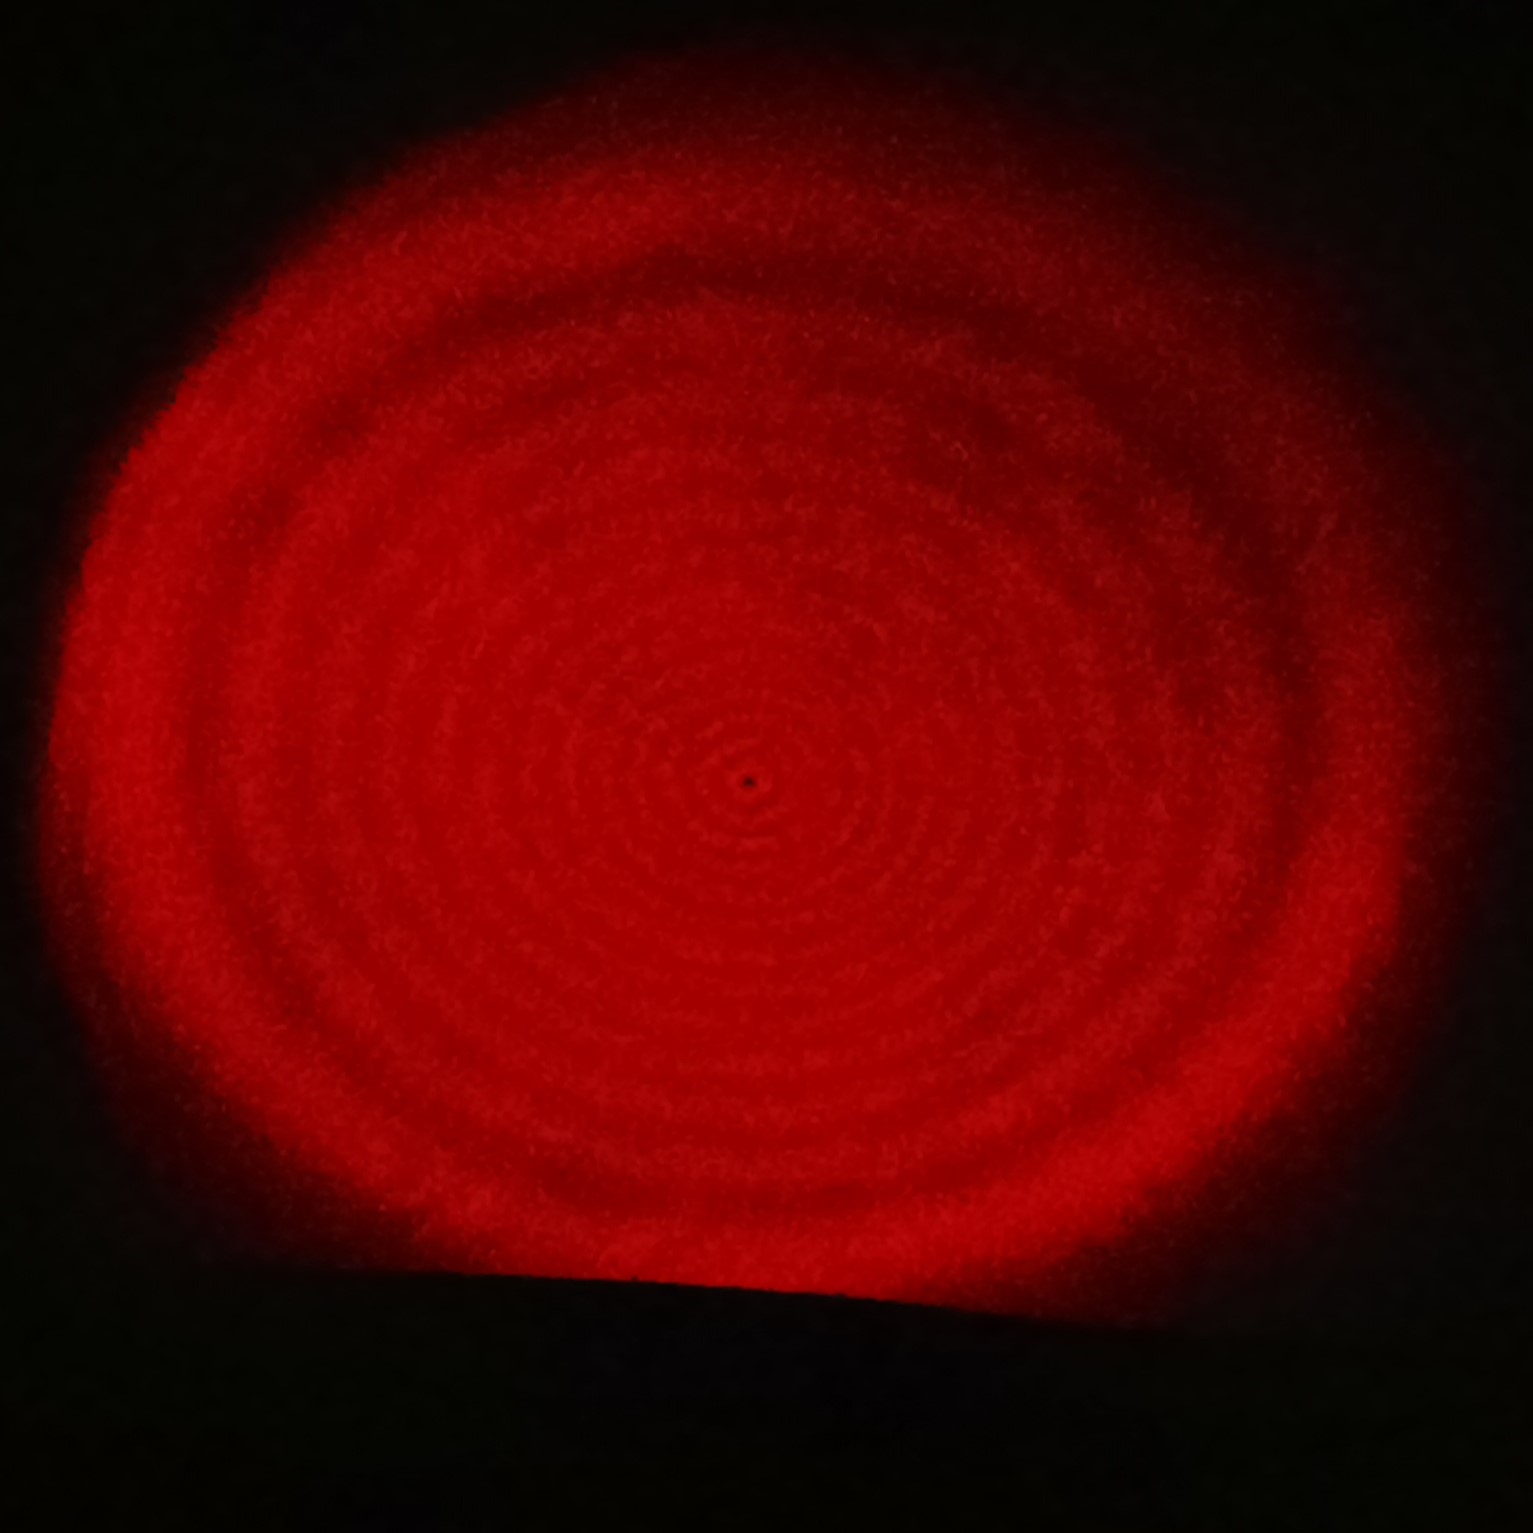
\includegraphics[width=0.3\linewidth]{../img/svazek-r.jpg}
        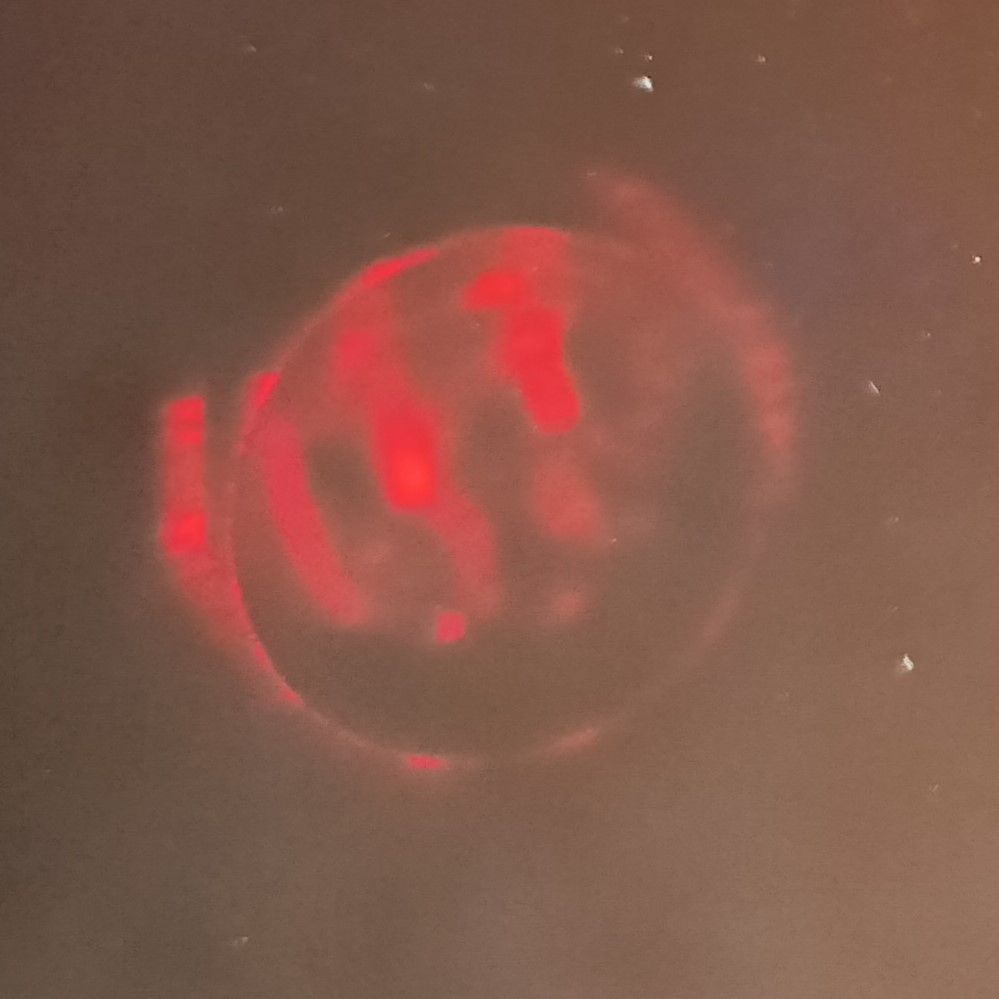
\includegraphics[width=0.3\linewidth]{../img/hologram-r-r.jpg}
        \label{img:svazky-r}
    }
    \subfigure[výkonová]{
        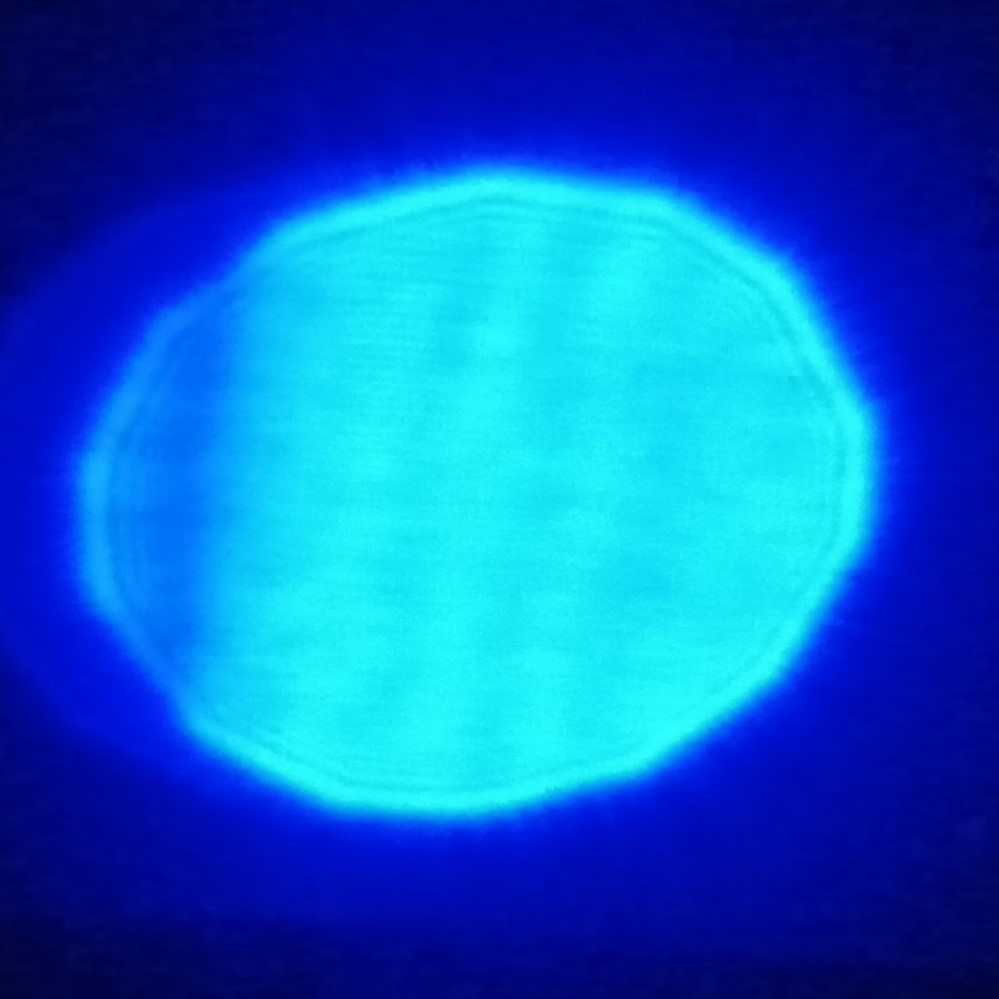
\includegraphics[width=0.3\linewidth]{../img/svazek-b.jpg}
        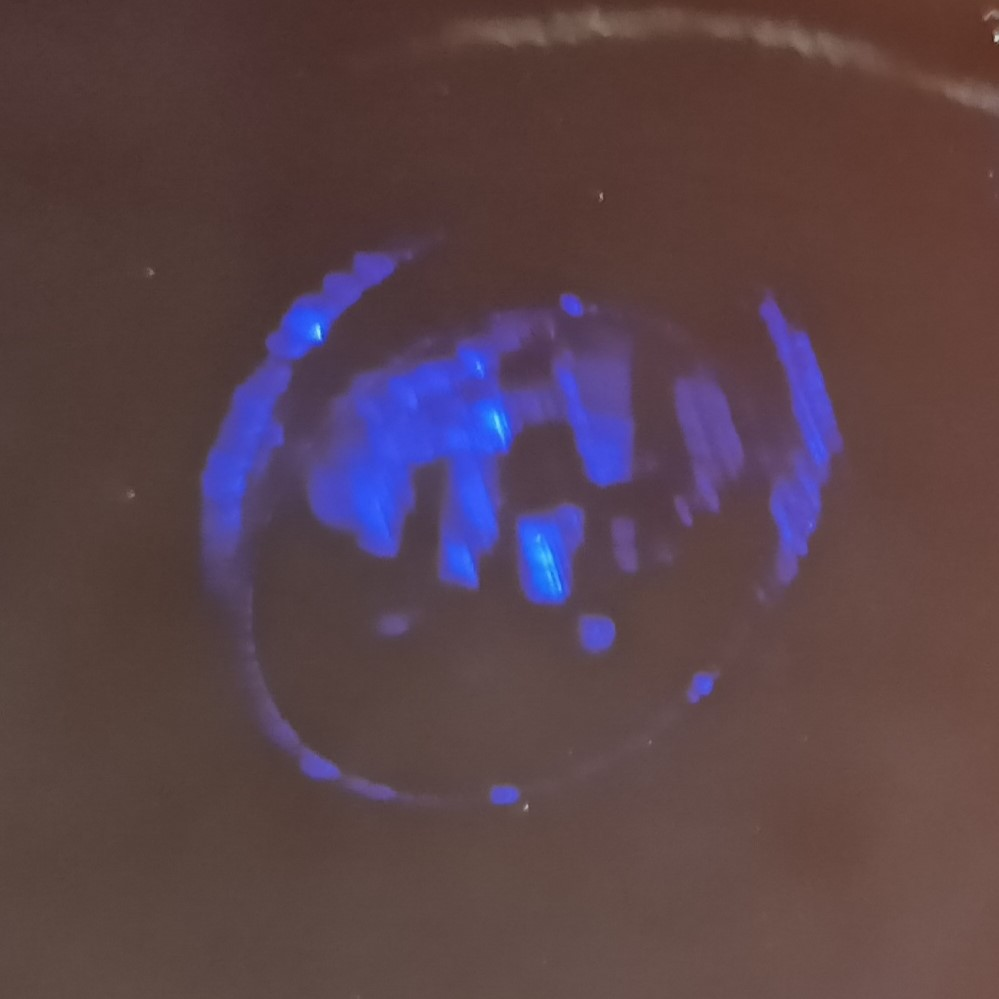
\includegraphics[width=0.3\linewidth]{../img/hologram-r-b.jpg}
        \label{img:svazky-b}
    }
    \caption{Vliv kvality svazku na výsledný hologram}
    \label{img:svazky}
\end{figure}

Červené světlo poskytl alignment laser o též dobrém tvaru svazku, rozložení intenzity zde však bylo konstantní a klasická geometrické optika na čočkách se tím pádem nechovala dle očekávání -- docházelo ke vzniku kroužků ve výsledné stopě. Tento jev je popisován v následující sekci \ref{sec:negauss}. Nominální světelný výkon tohoto laseru byl výrazně nižší, oproti předchozímu laseru pouchých $5\,\text{mW}$. Stopa i výsledný hologram jsou na obrázku \ref{img:svazky-r}.

Poslední složkou bylo modré světlo, pro které jsme využili výkonové laserové diody modré barvy. Tato dioda měla světelný výkon až $1\,\text{W}$, ovšem její svazek měl obdélníkový tvar a rozložení intenzity ve svazku bylo velmi různorodé. Oříznutí svazku a následná manipulace čočkami vedla na velmi nepěknou stopu a tedy i nekvalitní hologram na obrázku \ref{img:svazky-b}.

\medskip

Nejlepším zdrojem koherentního světla pro účely holografie by tedy byl solid-state laser, a to i přes nehomogenní, gaussovské, rozložení intenzity. Po dovyvolání holografické desky bílým světlem byl zelený hologram dokonce tak kvalitní a kontrastní, že na virtuální obraz bez problémů ostřilo automatické zasotření fotoaparátu mobilního telefonu. Tento holgoram tedy ještě jednou představujeme na obrázku \ref{img:hologram-refl}. % FIXME: Solid-State ???

\begin{figure}
    \centering
    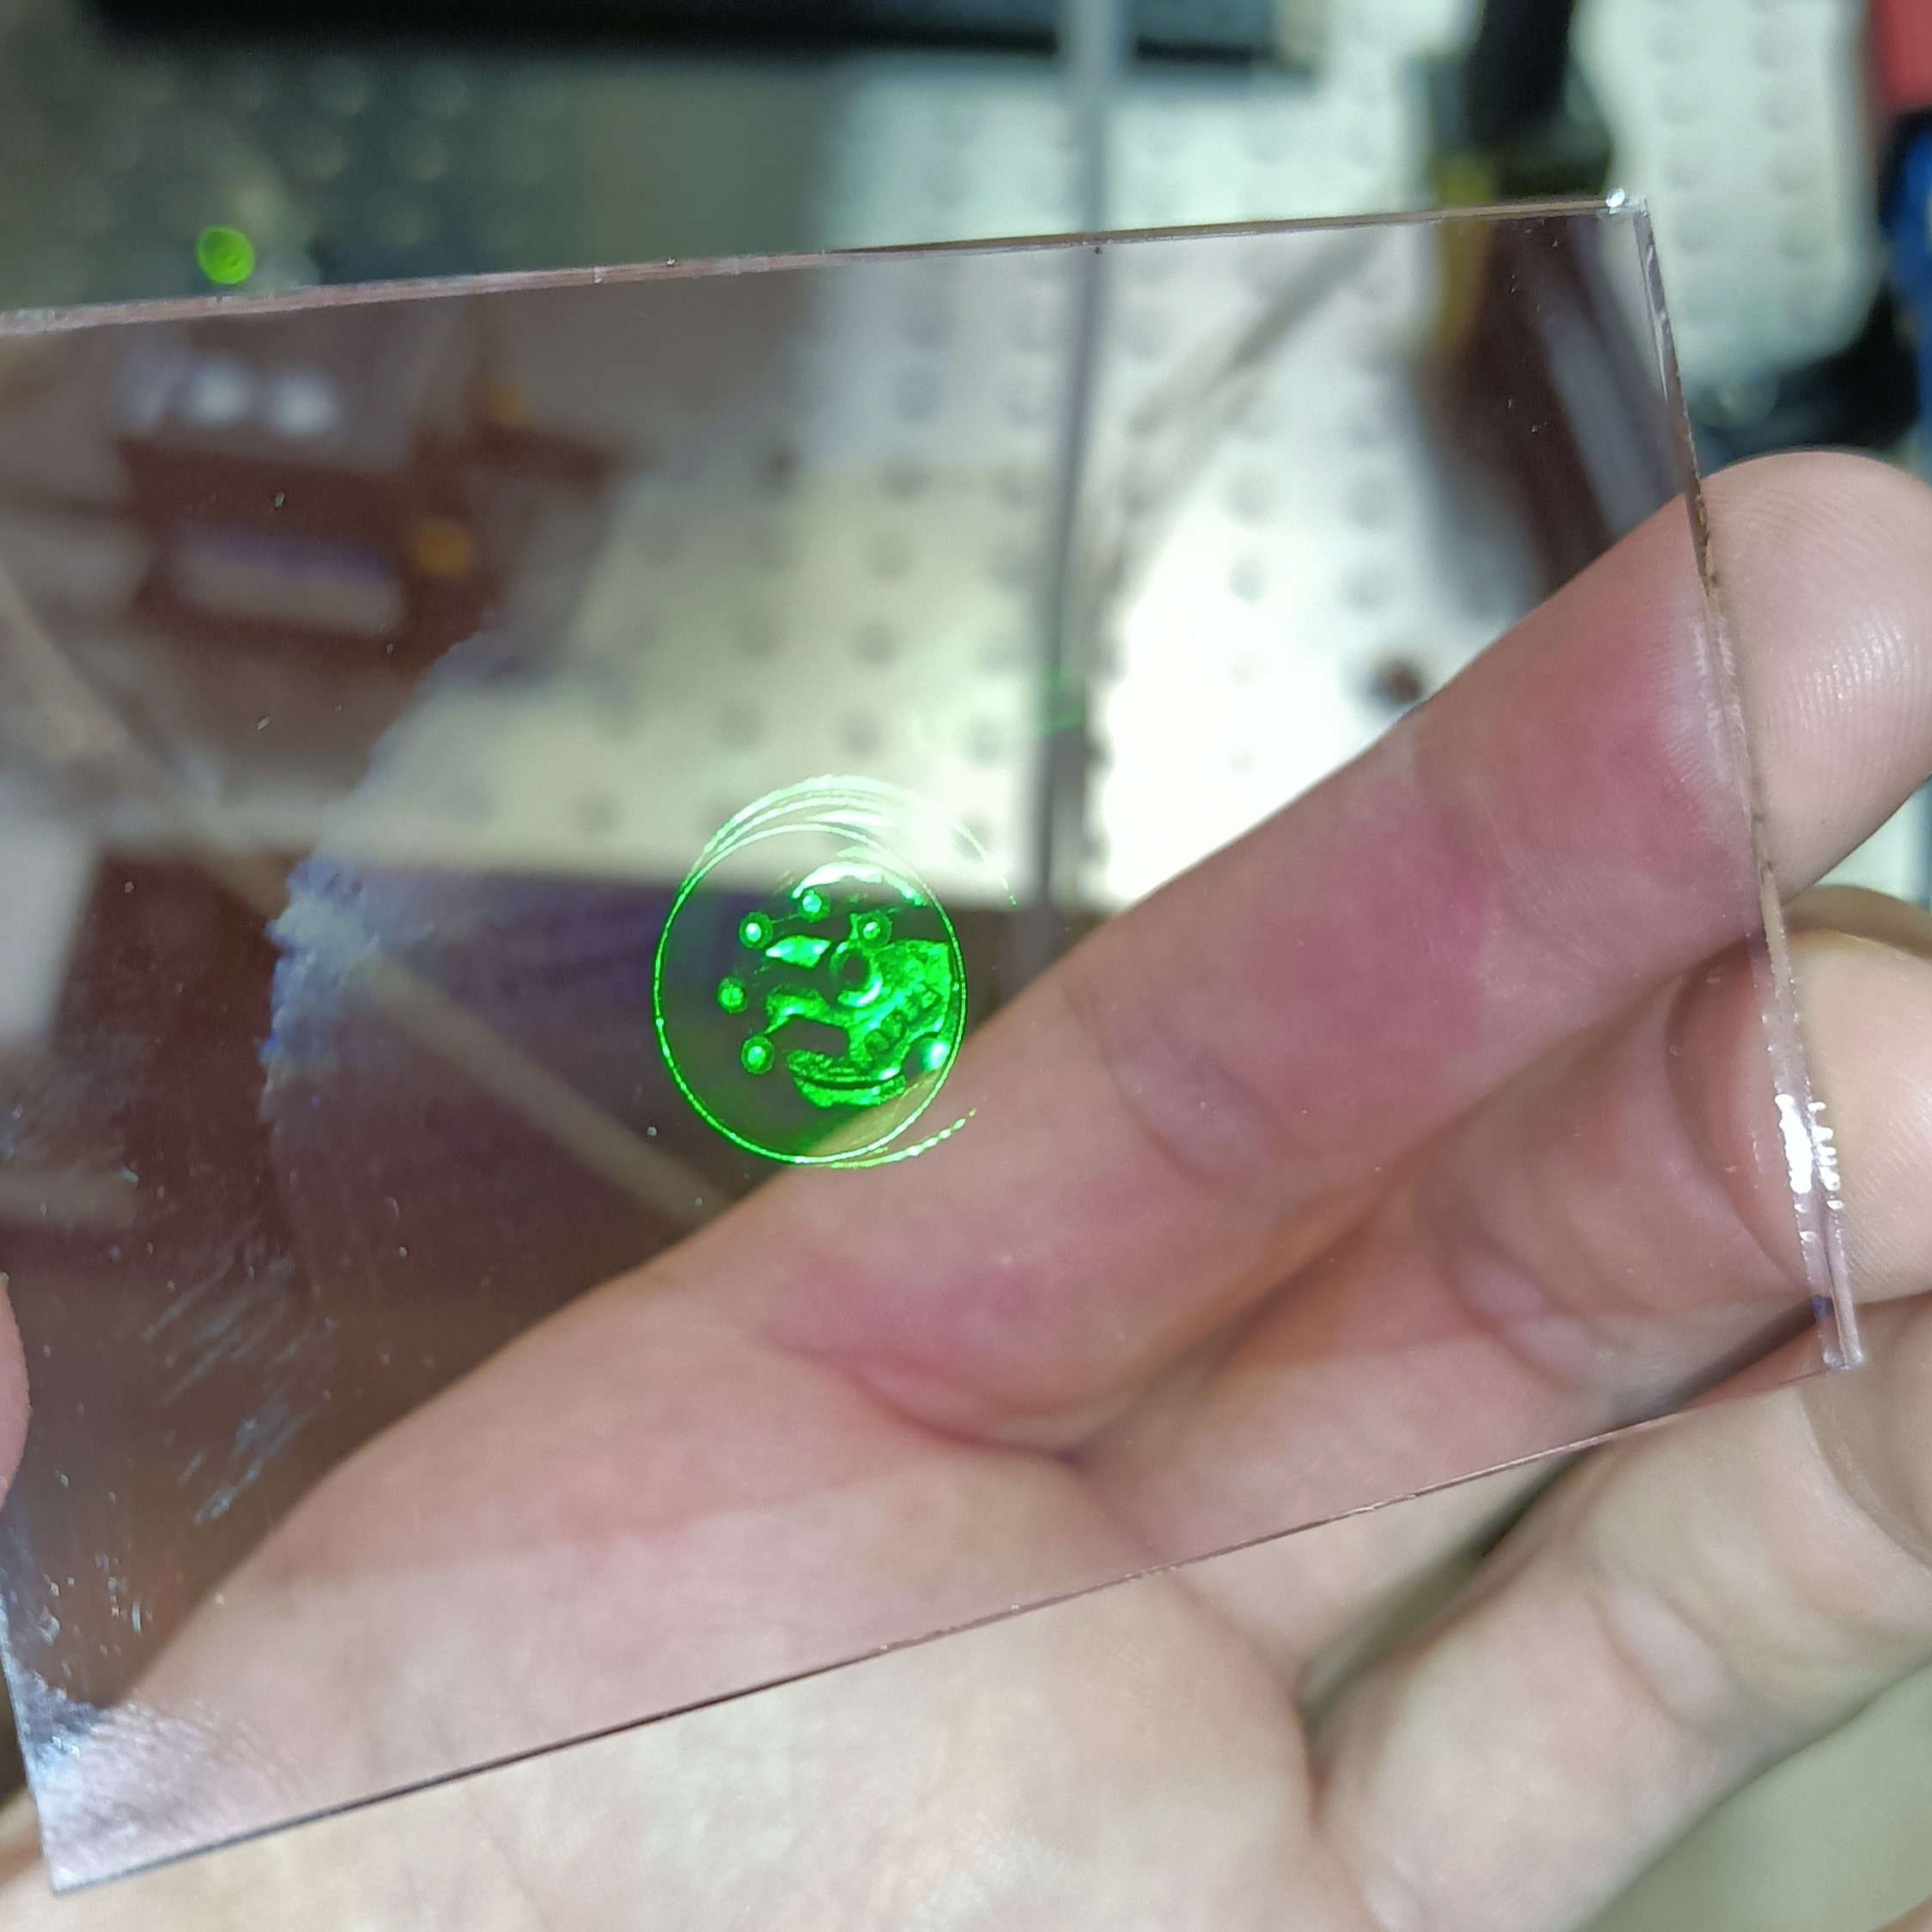
\includegraphics[width=0.6\linewidth]{../img/hologram-r-g2.jpg}
    \caption{Automaticky zaostřený reflexní hologram v zelené barvě}
    \label{img:hologram-refl}
\end{figure}

Tento typ laseru je však k dispozici pouze v této jedné vlnové délce a kombinovat různé druhy laserových zdrojů není vhodné. Velikost a způsob napájení tohoto laseru by navíc výrazně zhoršila přenosnost experimentálního uspořádání. Nakonec tedy byly pro nové uspořádání zvoleny alignment lasery, které jsou k dispozici ve červené, zelené i modré barvě a vyladěním nového uspořádání je možné kvalitu hologramu oproti tomuto pokusu zlepšit.

\subsection{Chování "`negaussovských"' svazků\label{sec:negauss}}
Pro pokrytí holografické desky a objektu je potřeba malý laserový svazek rozšířit na větší plochu (ve finálním uspořádání používáme kolem $60\,\text{cm}^2$). Toto jsme zprvu považovali za triviální, prostým vložením rozptylné čočky s vhodnou ohniskovou vzdáleností svazek zvětšíme na libovolnou plochu. Toto bez problémů funguje pro nekoherentní světlo a pro svazky koherentního světla s gaussovským rozložením intenzity toto opravdu platí bez problémů. U použitých alignment laserů však máme rovnoměrné rozložení intenzity (znázorněno na obrázku \ref{img:intenzity}), které způsobuje problémy.

\begin{figure}[!ht]
    \centering
    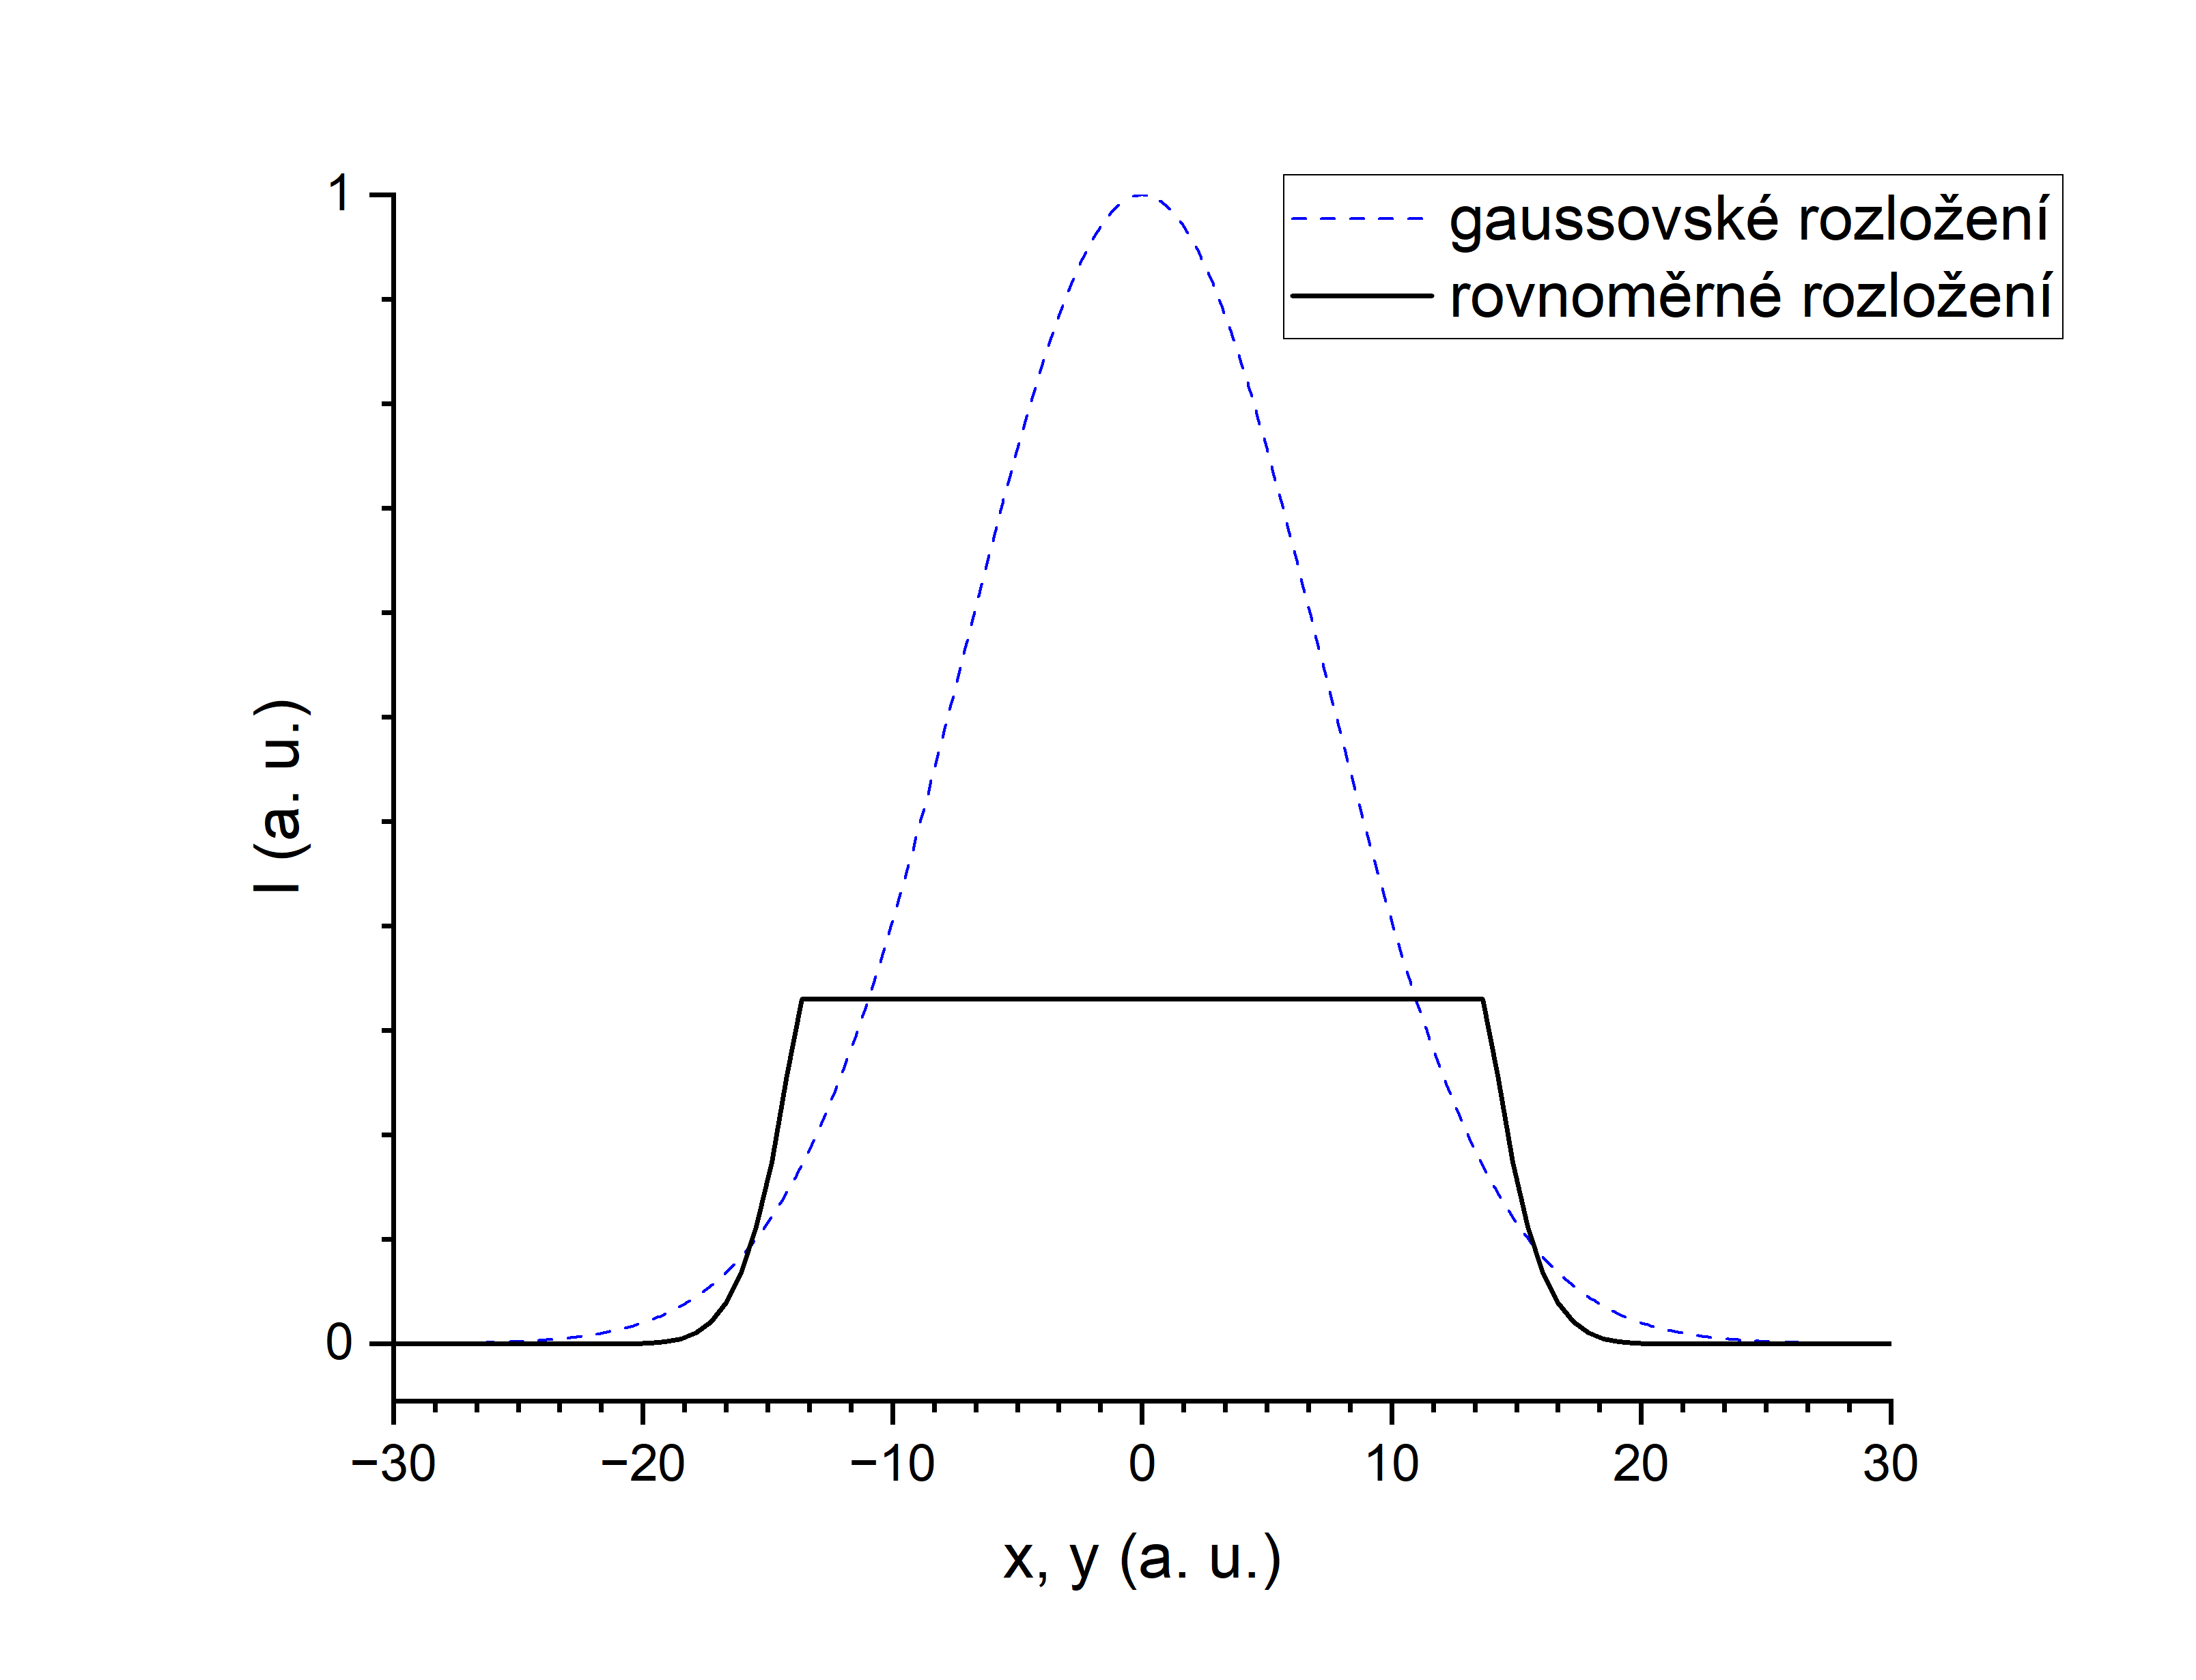
\includegraphics[width=0.6\linewidth]{../img/rozlozeni-intenzity.png}
    \caption{Ilustrace gaussovského a rovnoměrného rozložení intenzity ve svazku}
    \label{img:intenzity}
\end{figure}

Uvnitř reálných čoček dochází k vnitřním odrazům na stěnách čoček. To v případě nekoherentního světla pouze snižuje kvalitu obrazu, v případě koherentního světla ale dochází unitř čočky k interferenci procházejícího světla s vnitřními odrazy. Je-li rozložení intenzity ve svazku koherentního světla gaussovské, je interference potlačena, u jiných rozložení však vznikají interferenční obrazce, Airyovy kroužky, které jsou zřetelné na obrázku \ref{img:svazky-r} vlevo.

\medskip

Pro holografii je potřebné mít holografickou desku a objekt osvícené co nejvíce homogenním světlem, na což jsou svazky s rovnoměrným rozložením intenzity principiálně ideální, ovšem vznik interferenčních obrazců v čočkách narušuje homogenitu příliš na to, abychom mohli vyrábět hologramy přijatelné kvality. Z tohoto důvodu jsme se rozhodli nahradit čočky za dutá sférická a parabolická zrcadla.

Sférická a parabolická zrcadla mají stejně jako čočky danou ohniskovou vzdálenost a mají tedy možnost obraz zvětšovat. To navíc bez vnitřních odrazů. V případě sférického zrcadla by při přenosu obecného obrazu došlo k vnešení kulové vady, u parabolického zrcadla při správném nastavení nikoliv, ovšem jelikož přenášíme pouze homogenní laserový svazek, vady zobrazení nijak neovlivní výsledek.

Absence vnitřních odrazů znamená, že nedochází k interferenci a tedy vzniku interferenčních obrazců. Zde jsme bohužel opět narazili na úskalí reálných optických komponent: Použitá zrcadla mají na odrazivé vrstvě navíc ještě ochrannou vrstvu, která v našem případě efektivně vytvořila Fabryho-Pérotův interferometr, který vede na vznik dalších interferenčních obrazců. U parabolického zrcadla se dále stopa jevila tečkovaná, jev označovaný jako \textit{speckling}, ke kterému dochází při odrazu o hrubý povrch: Usuzujeme, že vzhledem k náročnosti vybrušování parabolických zrcadel je povrch tohoto zrcadla z výroby hrubší. Speckling je viditelný také na obrázku \ref{img:krouzky-parabolicke}.

\medskip

\begin{figure}
    \subfigure[parabolické zrcadlo]{
        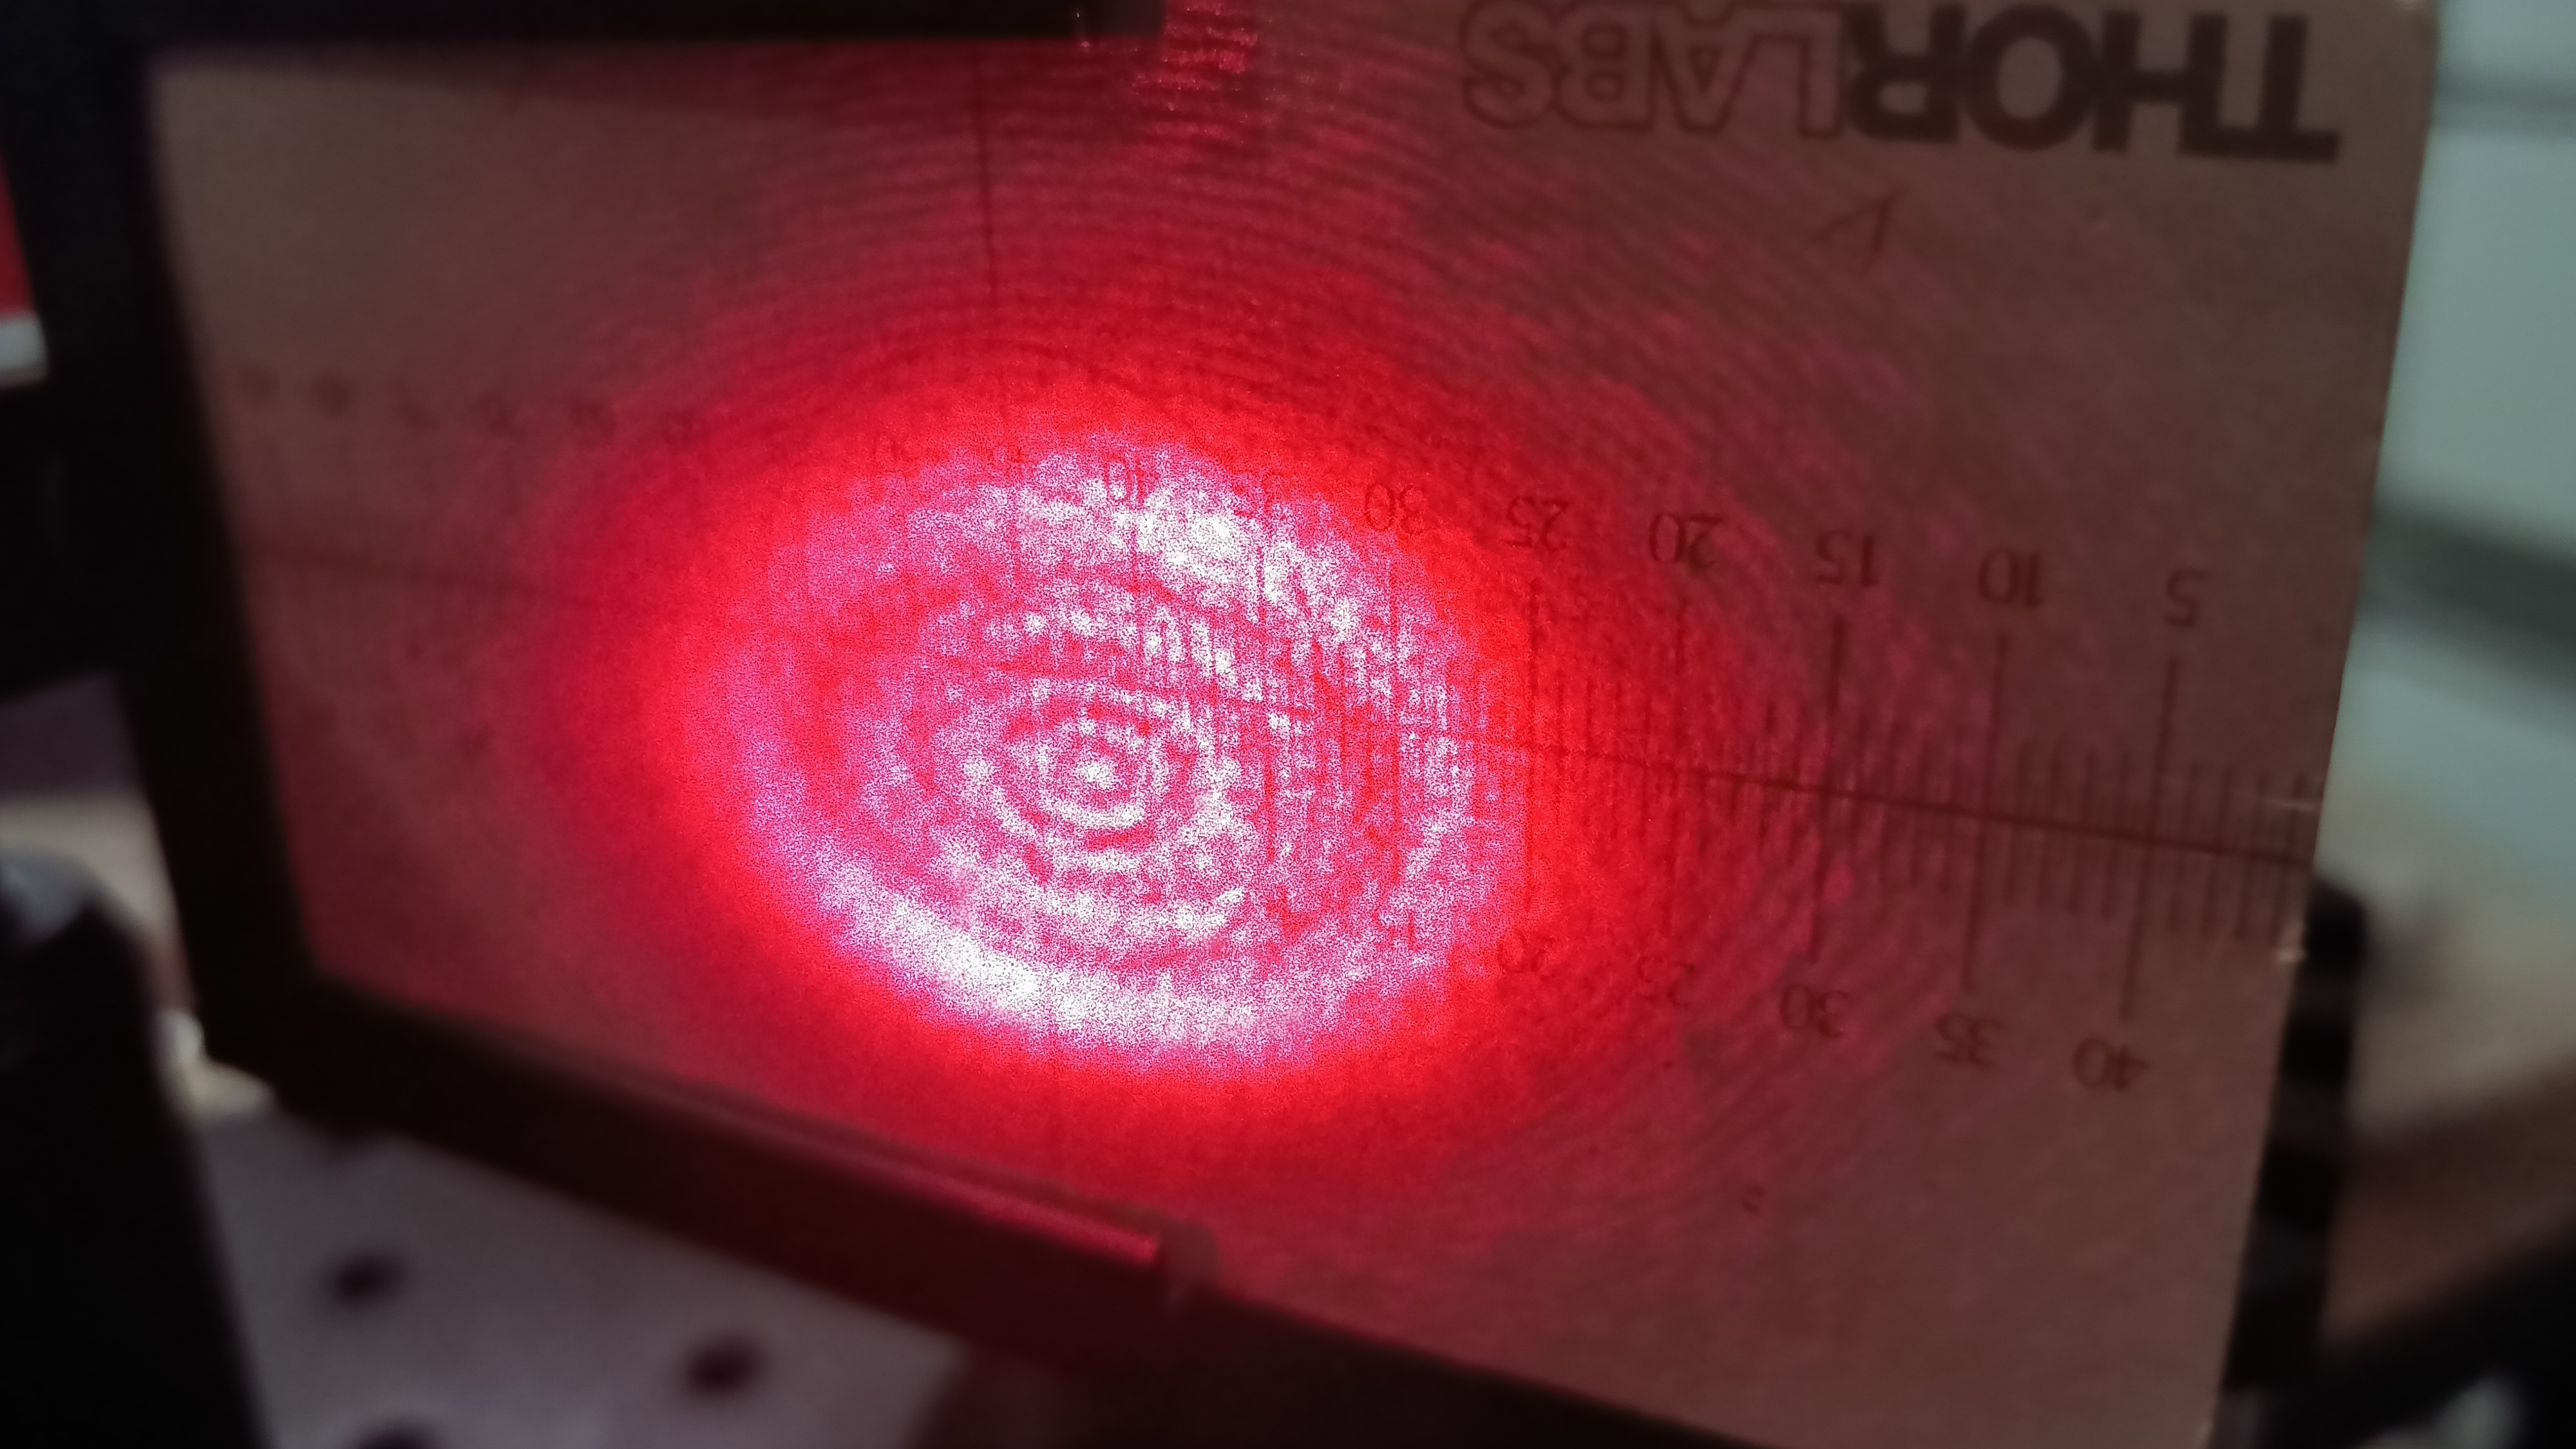
\includegraphics[width=0.4\linewidth]{../img/krouzky-parabolicke.jpg}
        \label{img:krouzky-parabolicke}
    }
    \hfill
    \subfigure[sférické zrcadlo]{
        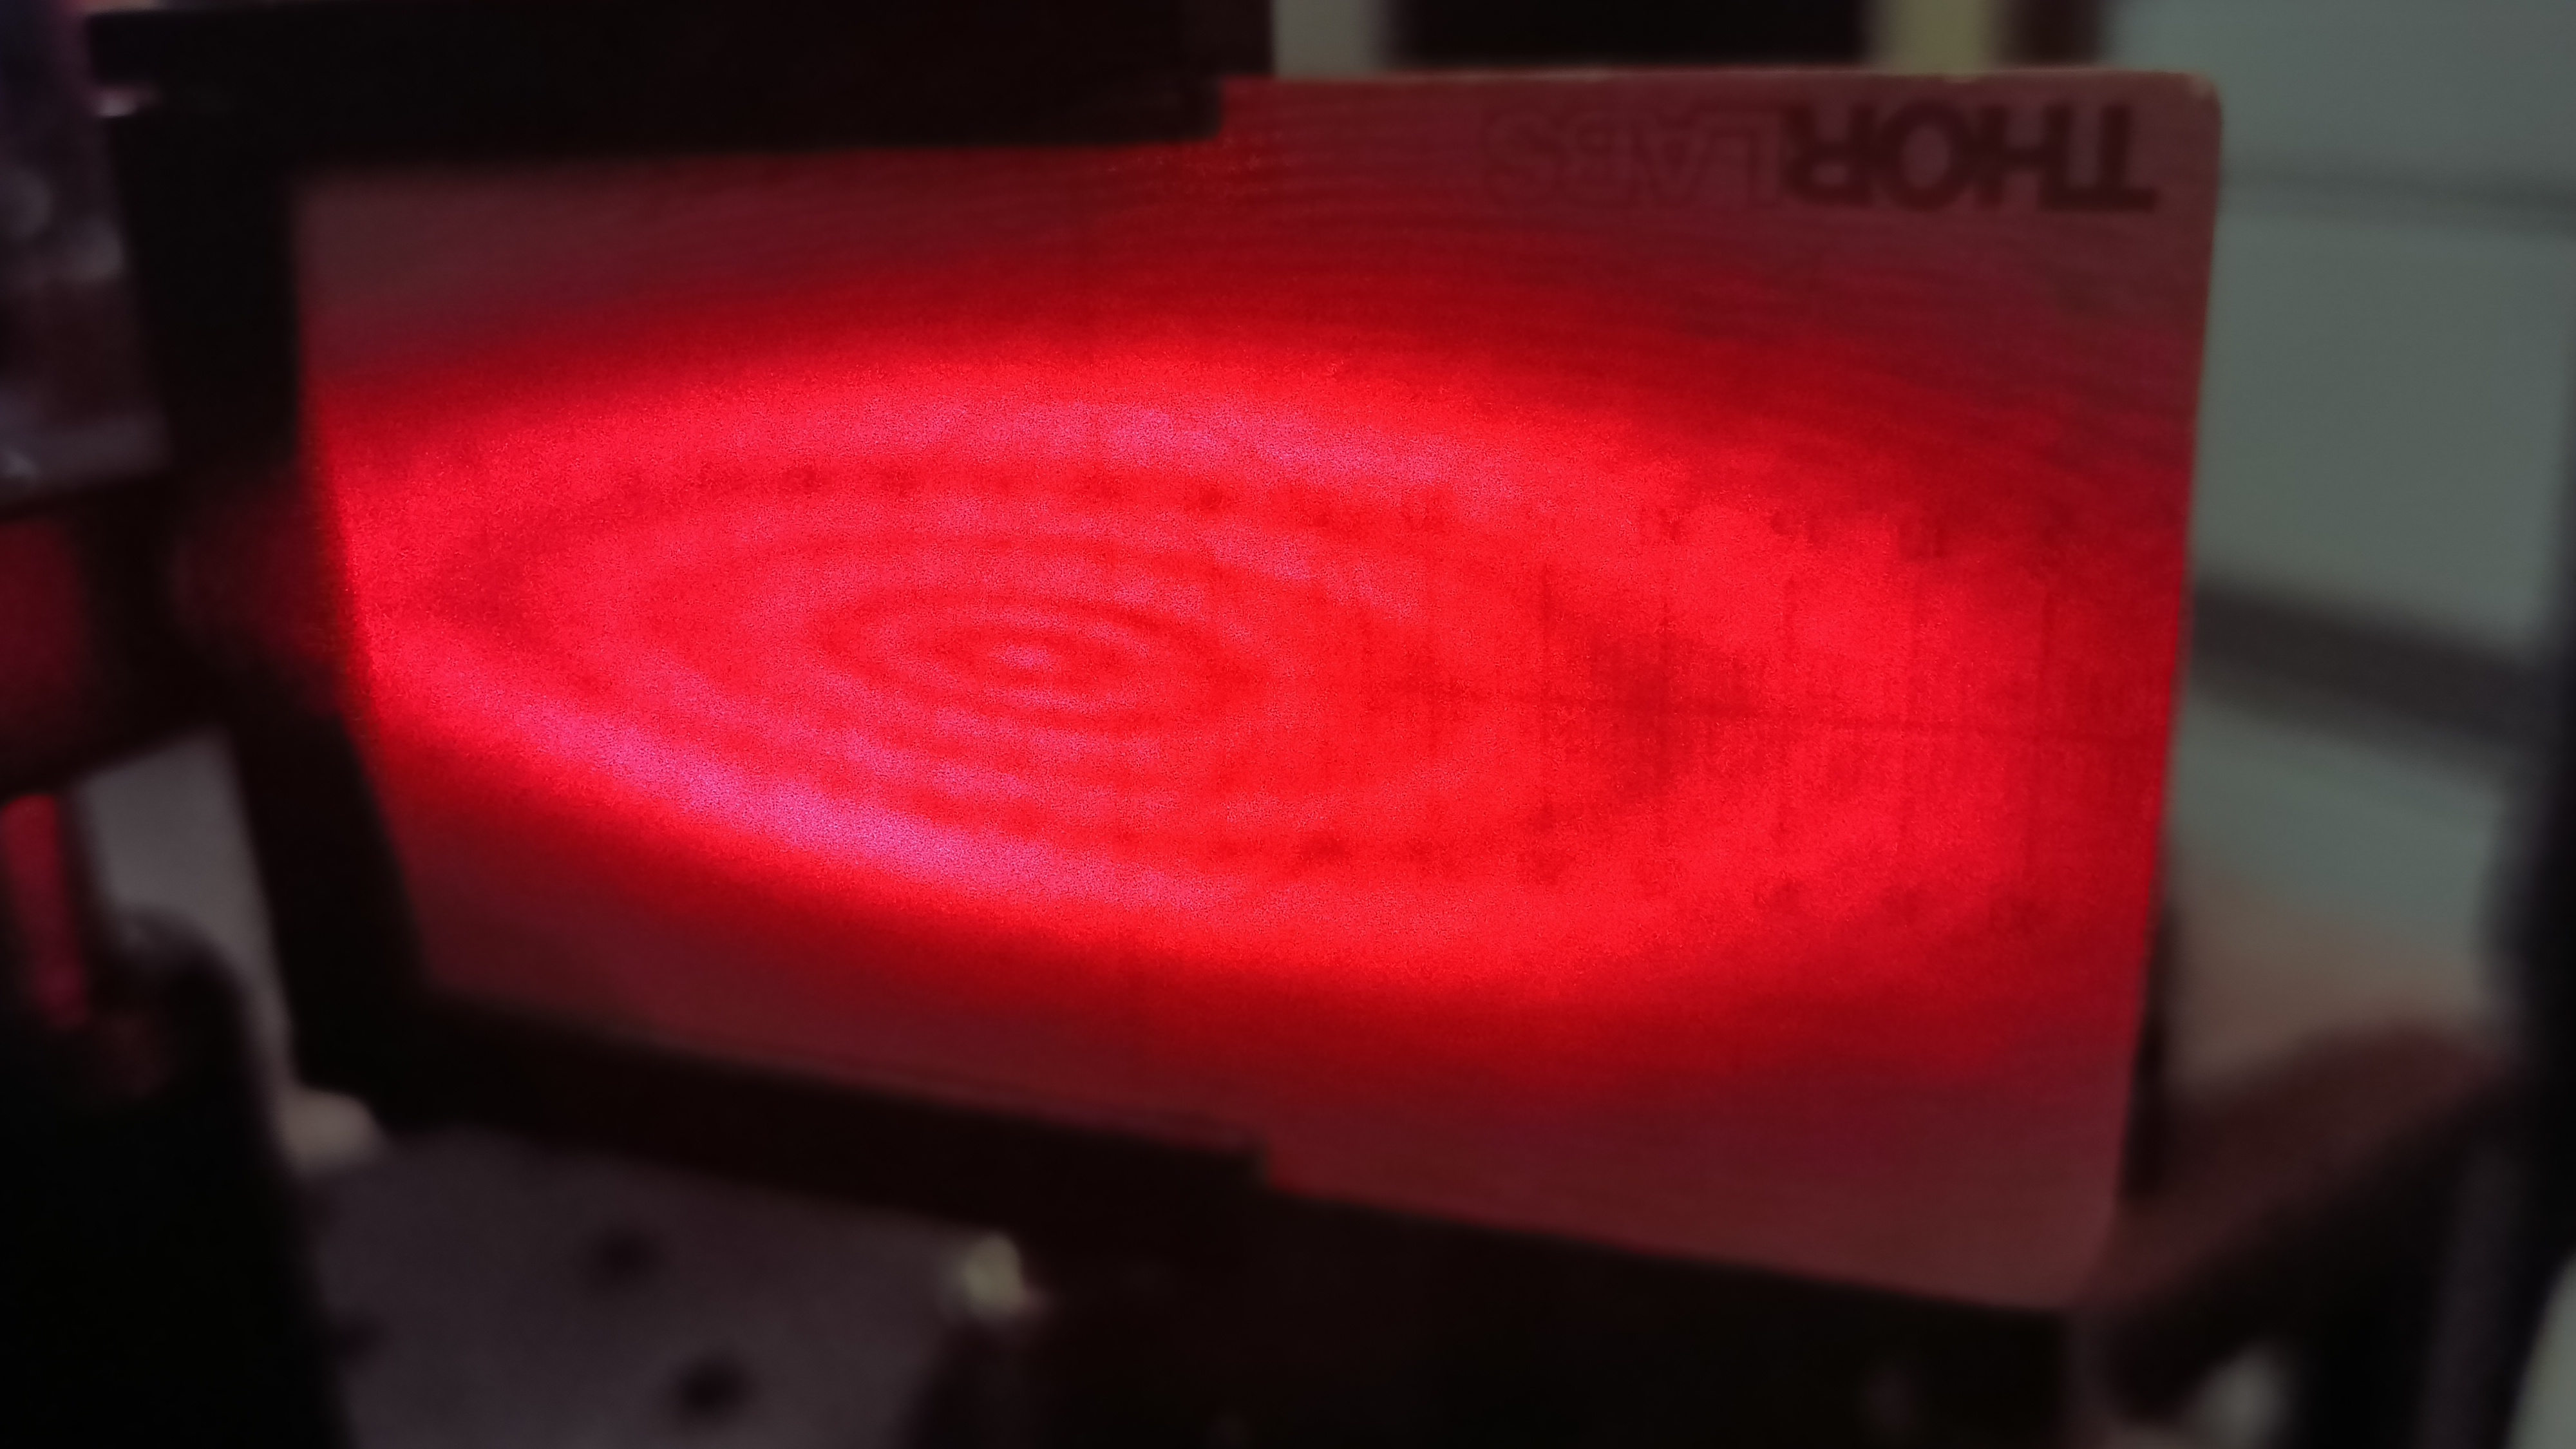
\includegraphics[width=0.4\linewidth]{../img/krouzky-sfericke.jpg}
    }
    \caption{Stopy laserového svazku po rozšíření parabolickým a sférickým zrcadlem}
    \label{img:krouzky}
\end{figure}

Ultimátním řešením by bylo použití buďto zrcadel bez ochranné vrstvy, která by se ale pravděpodobně velmi rychle poškodila, nebo použití zrcadel vypouklých, která ale bohužel výrobce námi používaných optických součástek nevyrábí. Pro rozšíření svazku dopadajícího na holografickou desku jsme proto zvolili sférické zrcadlo namísto původně preferovaného parabolického, jelikož při porovnání v obrázku \ref{img:krouzky} vedlo na méně ostré interferenční obrazce a při lehkém rozladění jednotlivých laserů vytvářelo přijatelně homogenní stopu téměř bílé barvy na obrázku \ref{img:bila}.

\begin{figure}
    \centering
    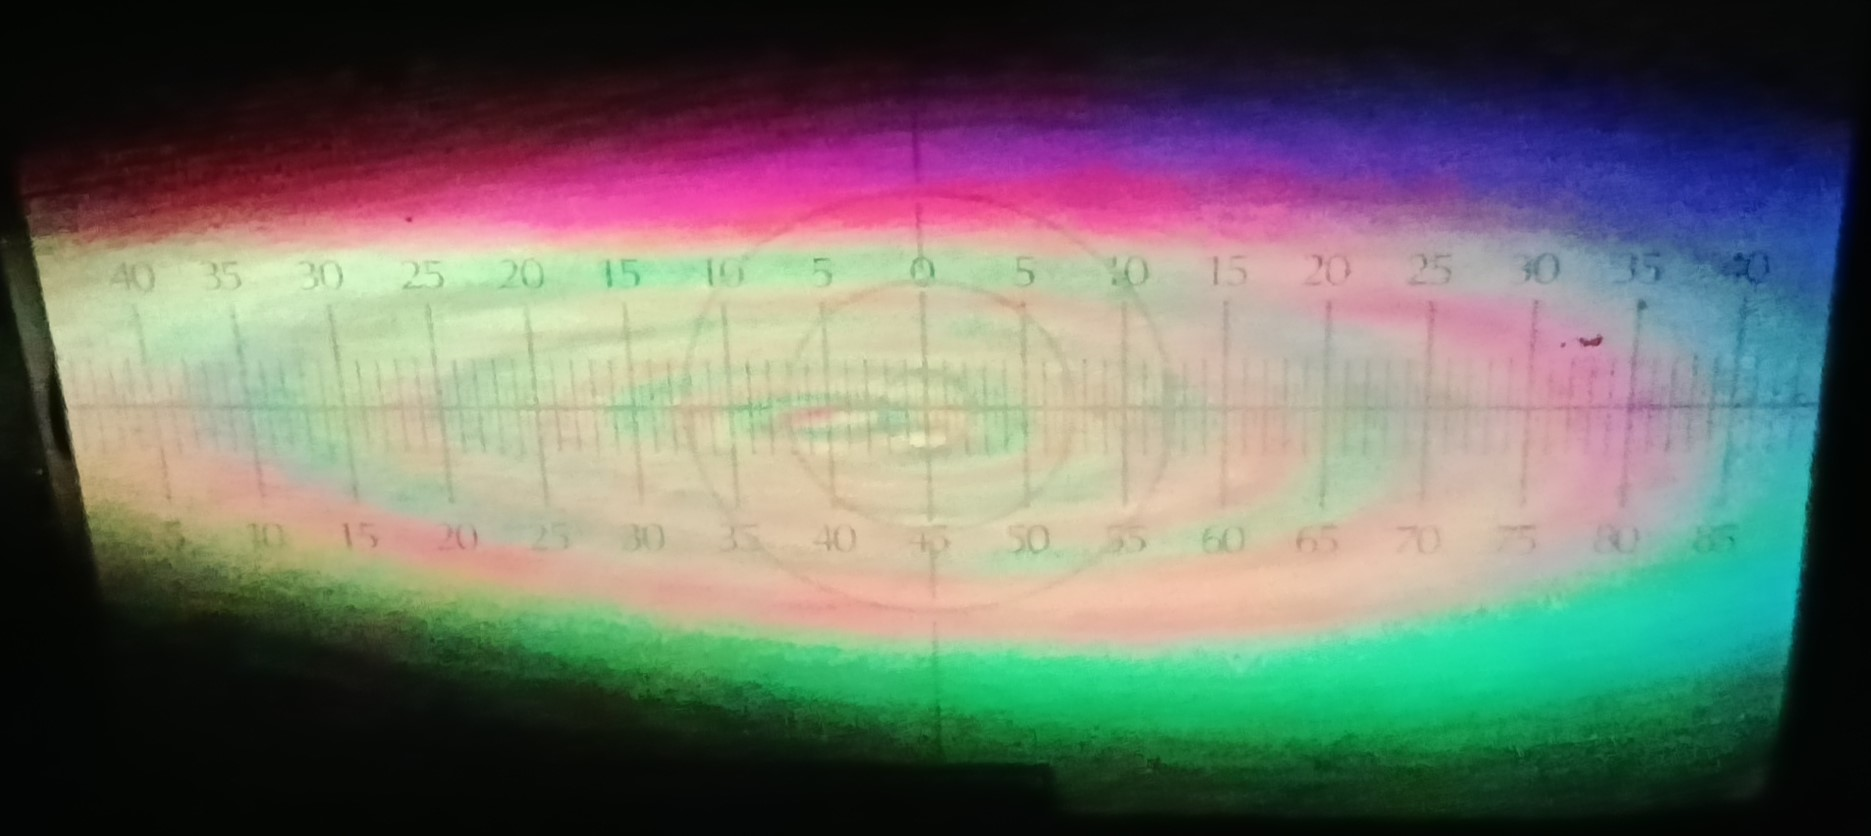
\includegraphics[width=0.7\linewidth]{../img/rgb-stopa.jpg}
    \caption{Stopa kombinace červeného, zeleného a modrého laserového svazku}
    \label{img:bila}
\end{figure}

\section{Vliv úhlu dopadu na holografickou desku}
Z teorie Fresnelovské optiky plyne, že při dopadu světla s $p$-polarizací na povrch pod Brewsterovým úhlem nedochází k odrazu světla. Jelikož pro holografii chceme odstranit jakékoli paprsky, které by mohly interferovat na holografické desce a způsobovat tak světelnou "`mlhu"' ve výsledném hologramu zvanou \textit{halo}, je vhodné splnit tyto podmínky: Brewsterův úhel a $p$-polarizaci.

Až do finálních úprav jsme se vskutku snažili Brewsterův úhel dodržovat, ovšem jelikož je tento úhel pro používané holografické desky mezi $50$ a $60^\circ$, byl stejný i pozorovací úhel výsledných hologramů. To znamenalo, že se člověk na hologram, obzvlášť v případě reflexních hologramů, musel dívat ze strany.

Při posledních pokusech jsme se rozhodli toto ignorovat a laserový paprsek na holografickou desku pustit téměř kolmo. Překvapivě se ukázalo, že halo nebylo nijak významné a pro pozorování byl hologram výrazně pohodlnější. Finální uspořádání tedy používá tento minimální úhel dopadu.

\vfill
\noindent
\textit{Následující kapitoly již dokumentují současný stav.}
\chapter{Optická část\label{cpt:optika}}
\begin{center}
    Tato kapitola je přehledovou dokumentací finálního stavu optického experimentálního uspořádání.

    Veškerá optická aparatura včetně trojice laserů je umístěna na desce, kterou lze jednoduše přesouvat. Disponuje magnetickým držákem pro zrcátko, jímž lze do soustavy navést externí laser, a pozicí pro vložení senzoru měřiče intenzity světla, která je potřeba pro výpočet doby expozice. Sestaveny byly také nový držák holografické desky a platforma pro umístění objektu, která lze jednoduše přesunout či naopak upevnit a obsahuje jednoduchý mechanismus pro upevnění vzorku.
\end{center}
\section{Experimentální uspořádání\label{sec:usporadani}}
\begin{figure}[ht]
    \centering
    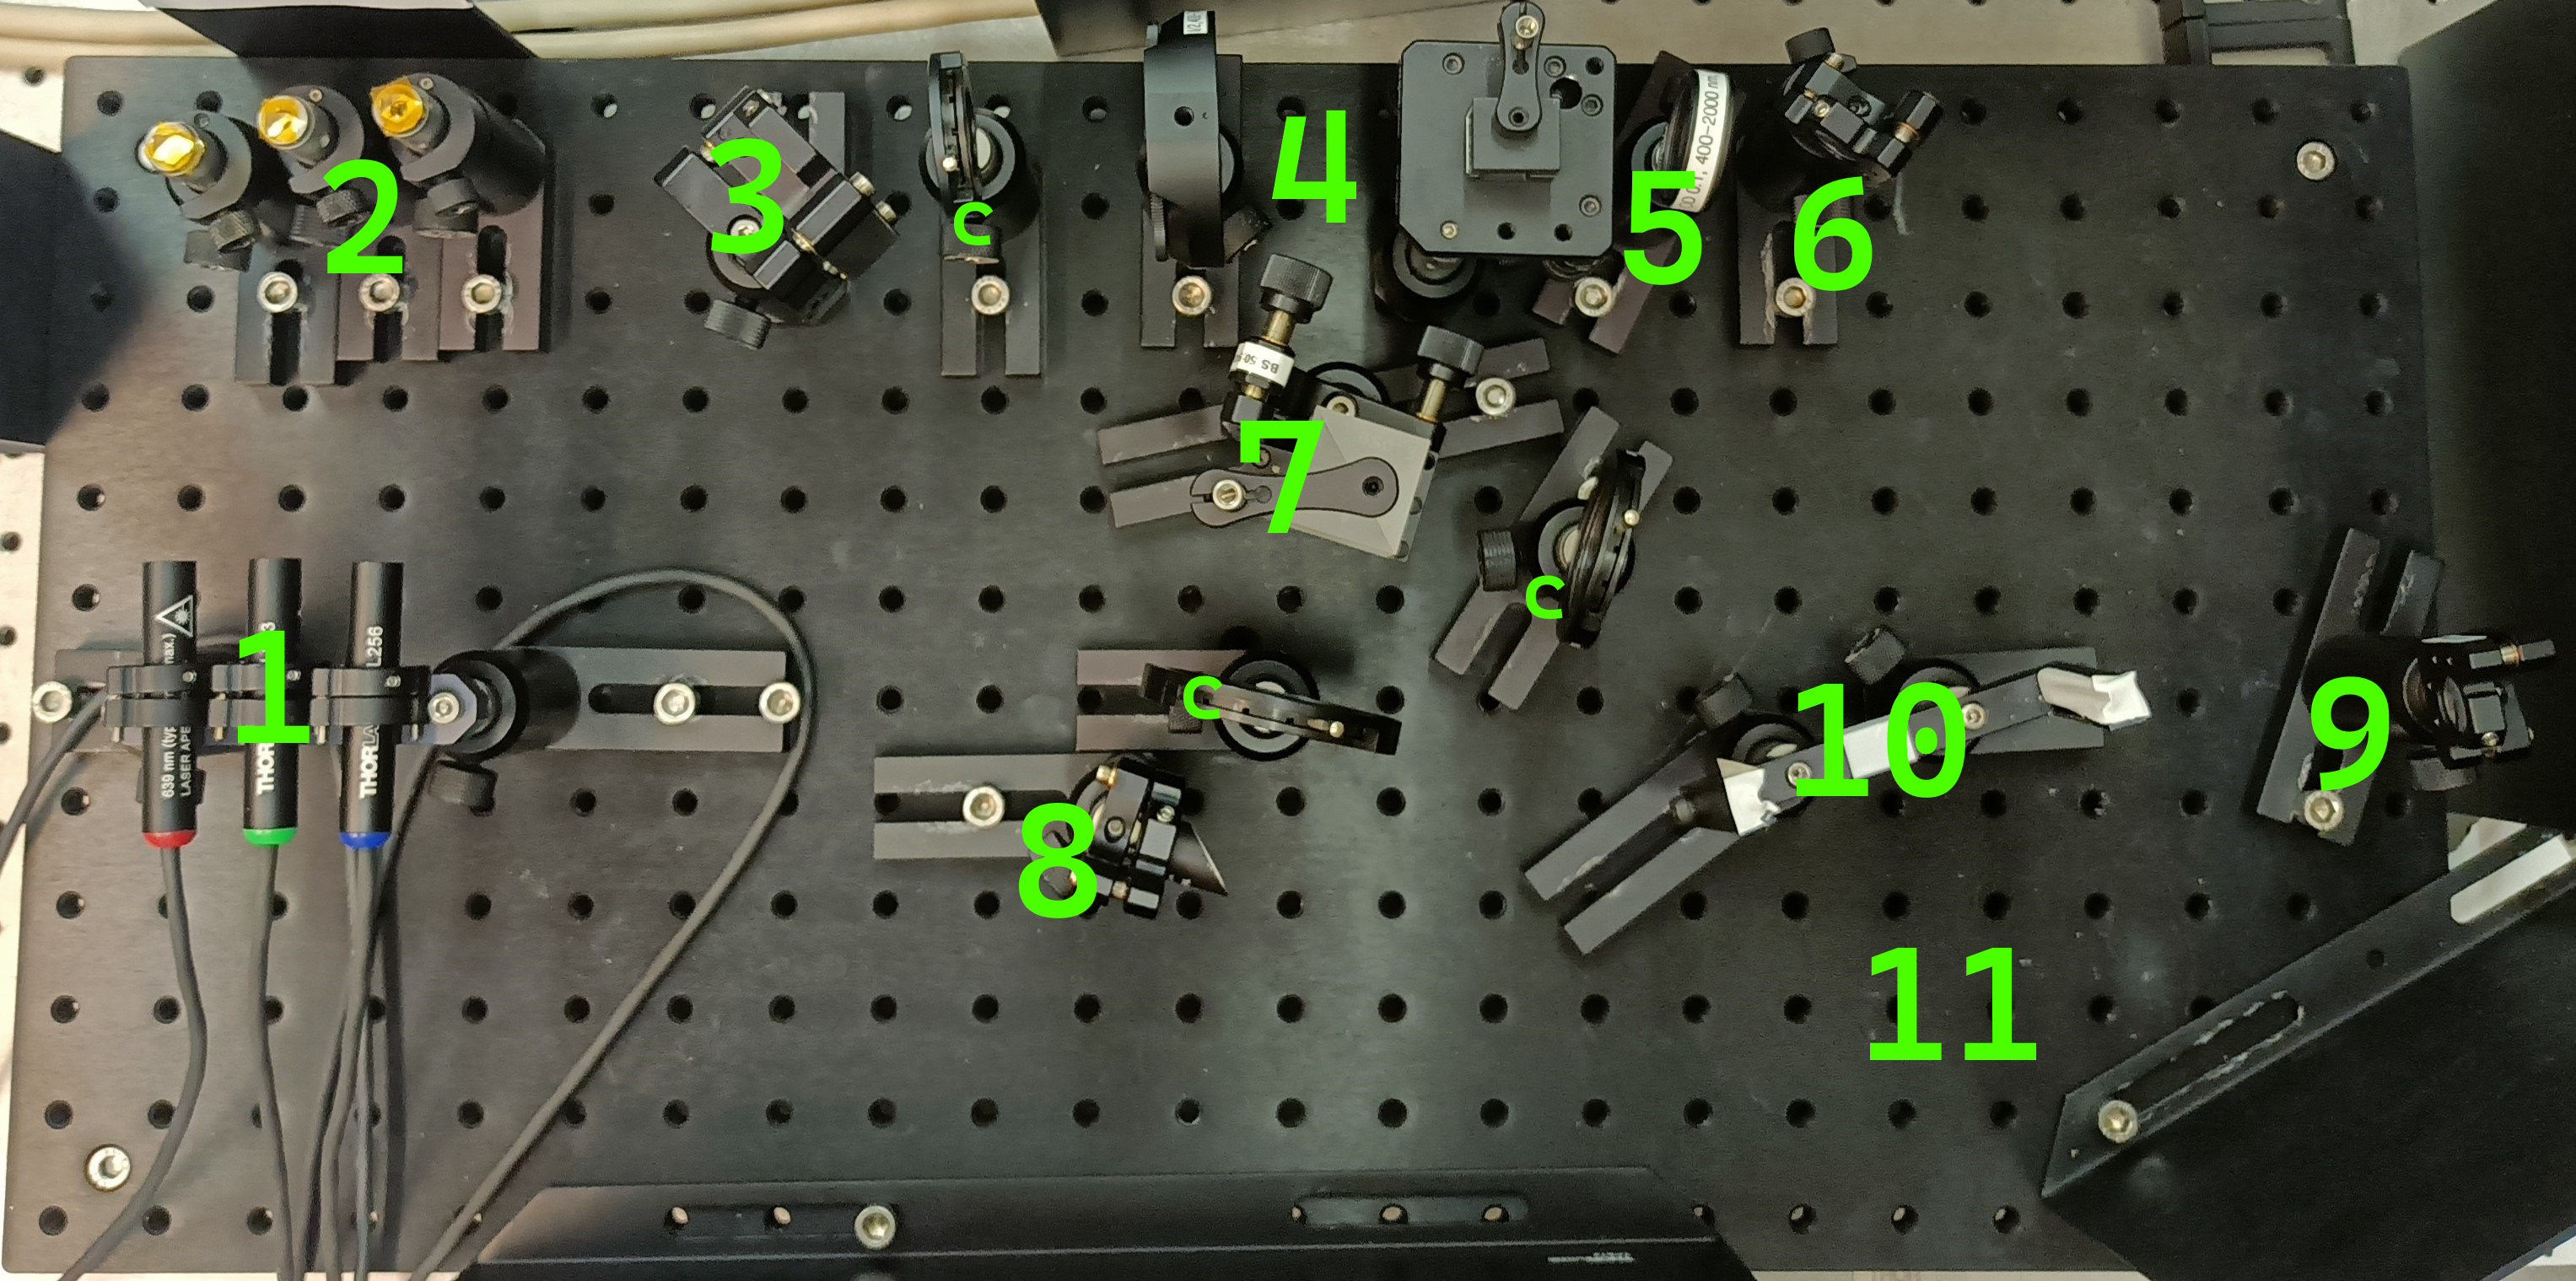
\includegraphics[width=\linewidth]{../img/nove-usporadani-popis.jpg}
    \caption{
        Popis nového experimentálního uspořádání:\\
        (\texttt{1}) trojice laserů, (\texttt{2}) malá rovinná zrcátka, (\texttt{3}) držák pro zrcadlo navádějící externí laser, (\texttt{4}) kombinace půlvlnové destičky a polarizačního děliče svazku, (\texttt{5}) pozice pro umístění senzoru, (\texttt{6}) sfériceké zrcadlo referenční vlny, (\texttt{7}) hranolový dělič objektové vlny, (\texttt{8}) parabolické zrcadlo pravé objektové vlny, (\texttt{9}) sférické zrcadlo levé objektové vlny, (\texttt{10}) držák holografické desky, (\texttt{11}) plocha pro umístění držáku objektu (nevyobrazen), (\texttt{c}) irisové clonky
    }
    \label{img:nove-usporadani-popis}
\end{figure}
Obrázek \ref{img:nove-usporadani-popis} ukazuje finální stav nového experimentálního uspořádání. Lasery (\texttt{1}) směřují na malá stříbrná rovinná zrcátka (\texttt{2}), která jsou blízko u sebe a tím navádějí trojici laserových svazků blízko u sebe. Kombinace půlvlnové destičky a polarizačního děliče svazků (\texttt{4}) umožňuje nastavit poměr intenzity referenční a objektové vlny, či pro reflexní uspořádání nasměrovat veškerou intenzitu na holografickou desku. Sférické zrcadlo (\texttt{6}) s ohniskovou vzdálenosti $9\,\text{mm}$ odráží a zvětšuje svazek na holografickou desku uchycenou v držáku (\texttt{10}) tak, že dopadá pod malým úhlem. Hranolový dělič svazků (\texttt{7}) rovnoměrně rozděluje svazek objektové vlny do dvou ramen, aby hologramy v transmisním uspořádání měly více pozorovacích úhlů. Parabolické zrcadlo (\texttt{8}) s ohniskovou vzdálenosti $9{,}5\,\text{mm}$ a sférické zrcadlo (\texttt{9}) s ohniskovou vzdáleností $12\,\text{mm}$ zvětšují ramena objektové vlny a odrážejí je na objekt, který je umístěn na podstaci v oblasti (\texttt{11}). Podstavec zde není vyobrazen, je však na obrázku \ref{img:prvni-iterace}. V uspořádání jsou také tři irisové clony (\texttt{c}), které slouží pro kalibraci a pro odstínění nežádoucích odrazů. Pravá dolní část uspořádání je také zastíněna několika černými stínítky pro zabránění úniku do a odrazu v prostoru laboratoře.

Jako zdroje koherentního světla (\texttt{1}) jsme zvolili alignment lasery, které jsou dostupné v červené, zelené a modré barvě a poskytují dle experimentů \ref{img:svazky-r} při lepším naladění rozumné výsledky. Jejich nevýhodou je, že jsou vyráběny pro účel čistě vizuální indikace, a tedy se při jejich výrobě příliš nedbá na přesnost vlnové délky. Modrý laser, který jehož nominální vlnová délka $420\,\text{nm}$ se již tak liší od vlnové délky $450\,\text{nm}$, na kterou je holografická deska v modré oblasti nejcitlivější, z výroby přišel s vlnovou délkou $402{,}1\,\text{nm}$, což je již na hranici ultrafialové oblasti světla a nejenže je na tuto vlnovou délku holografická deska velmi málo citlivá, optické komponenty pro viditelnou oblast na této vlnové délce již nemusí fungovat správně (např. zrcátka (\texttt{2}) mají pro tento konkrétní laser ztráty až $20\,\%$).

Držák (\texttt{3}) umožňuje magnetické uchycení rovinného zrcadla, pomocí kterého lze do aparatury navést externí laser. Vzhledem k malému světelnému výkonu napevno umístěných laserů (\texttt{1}), který je příliš nízky pro transmisní holografii při rozumných expozičních časech, budou transmisní hologramy vytvářeny pomocí externího laseru, např. dříve využívaného solid-state laseru, se kterým jsme i transmisní hologram vytvořili. Projekce tohoto transmisního hologramu je na obrázku \ref{img:transmisni}. % FIXME: Solid-State ???

Pozice (\texttt{5}) je primárně určena pro umístění senzoru měřiče intenzity světla, jejíž hodnota je potřeba pro výpočet expoziční doby (podrobněji popsáno v sekci \ref{sec:vyroba-hologramu}). Na obrázku \ref{img:nove-usporadani-popis} je v této pozici umístěn šedý filtr, který může být v závislosti na použítém externím laseru potřeba pro dodatečné snížení intenzity referenční vlny v transmisní holografii pro dasažení správného poměru referenční a objektové vlny (k tomu nemusí stačit polarizační dělič, který při eliptické polarizaci světla propustí v minimu větší intenzitu, než je žádoucí).

\begin{figure}[htp]
    \centering
    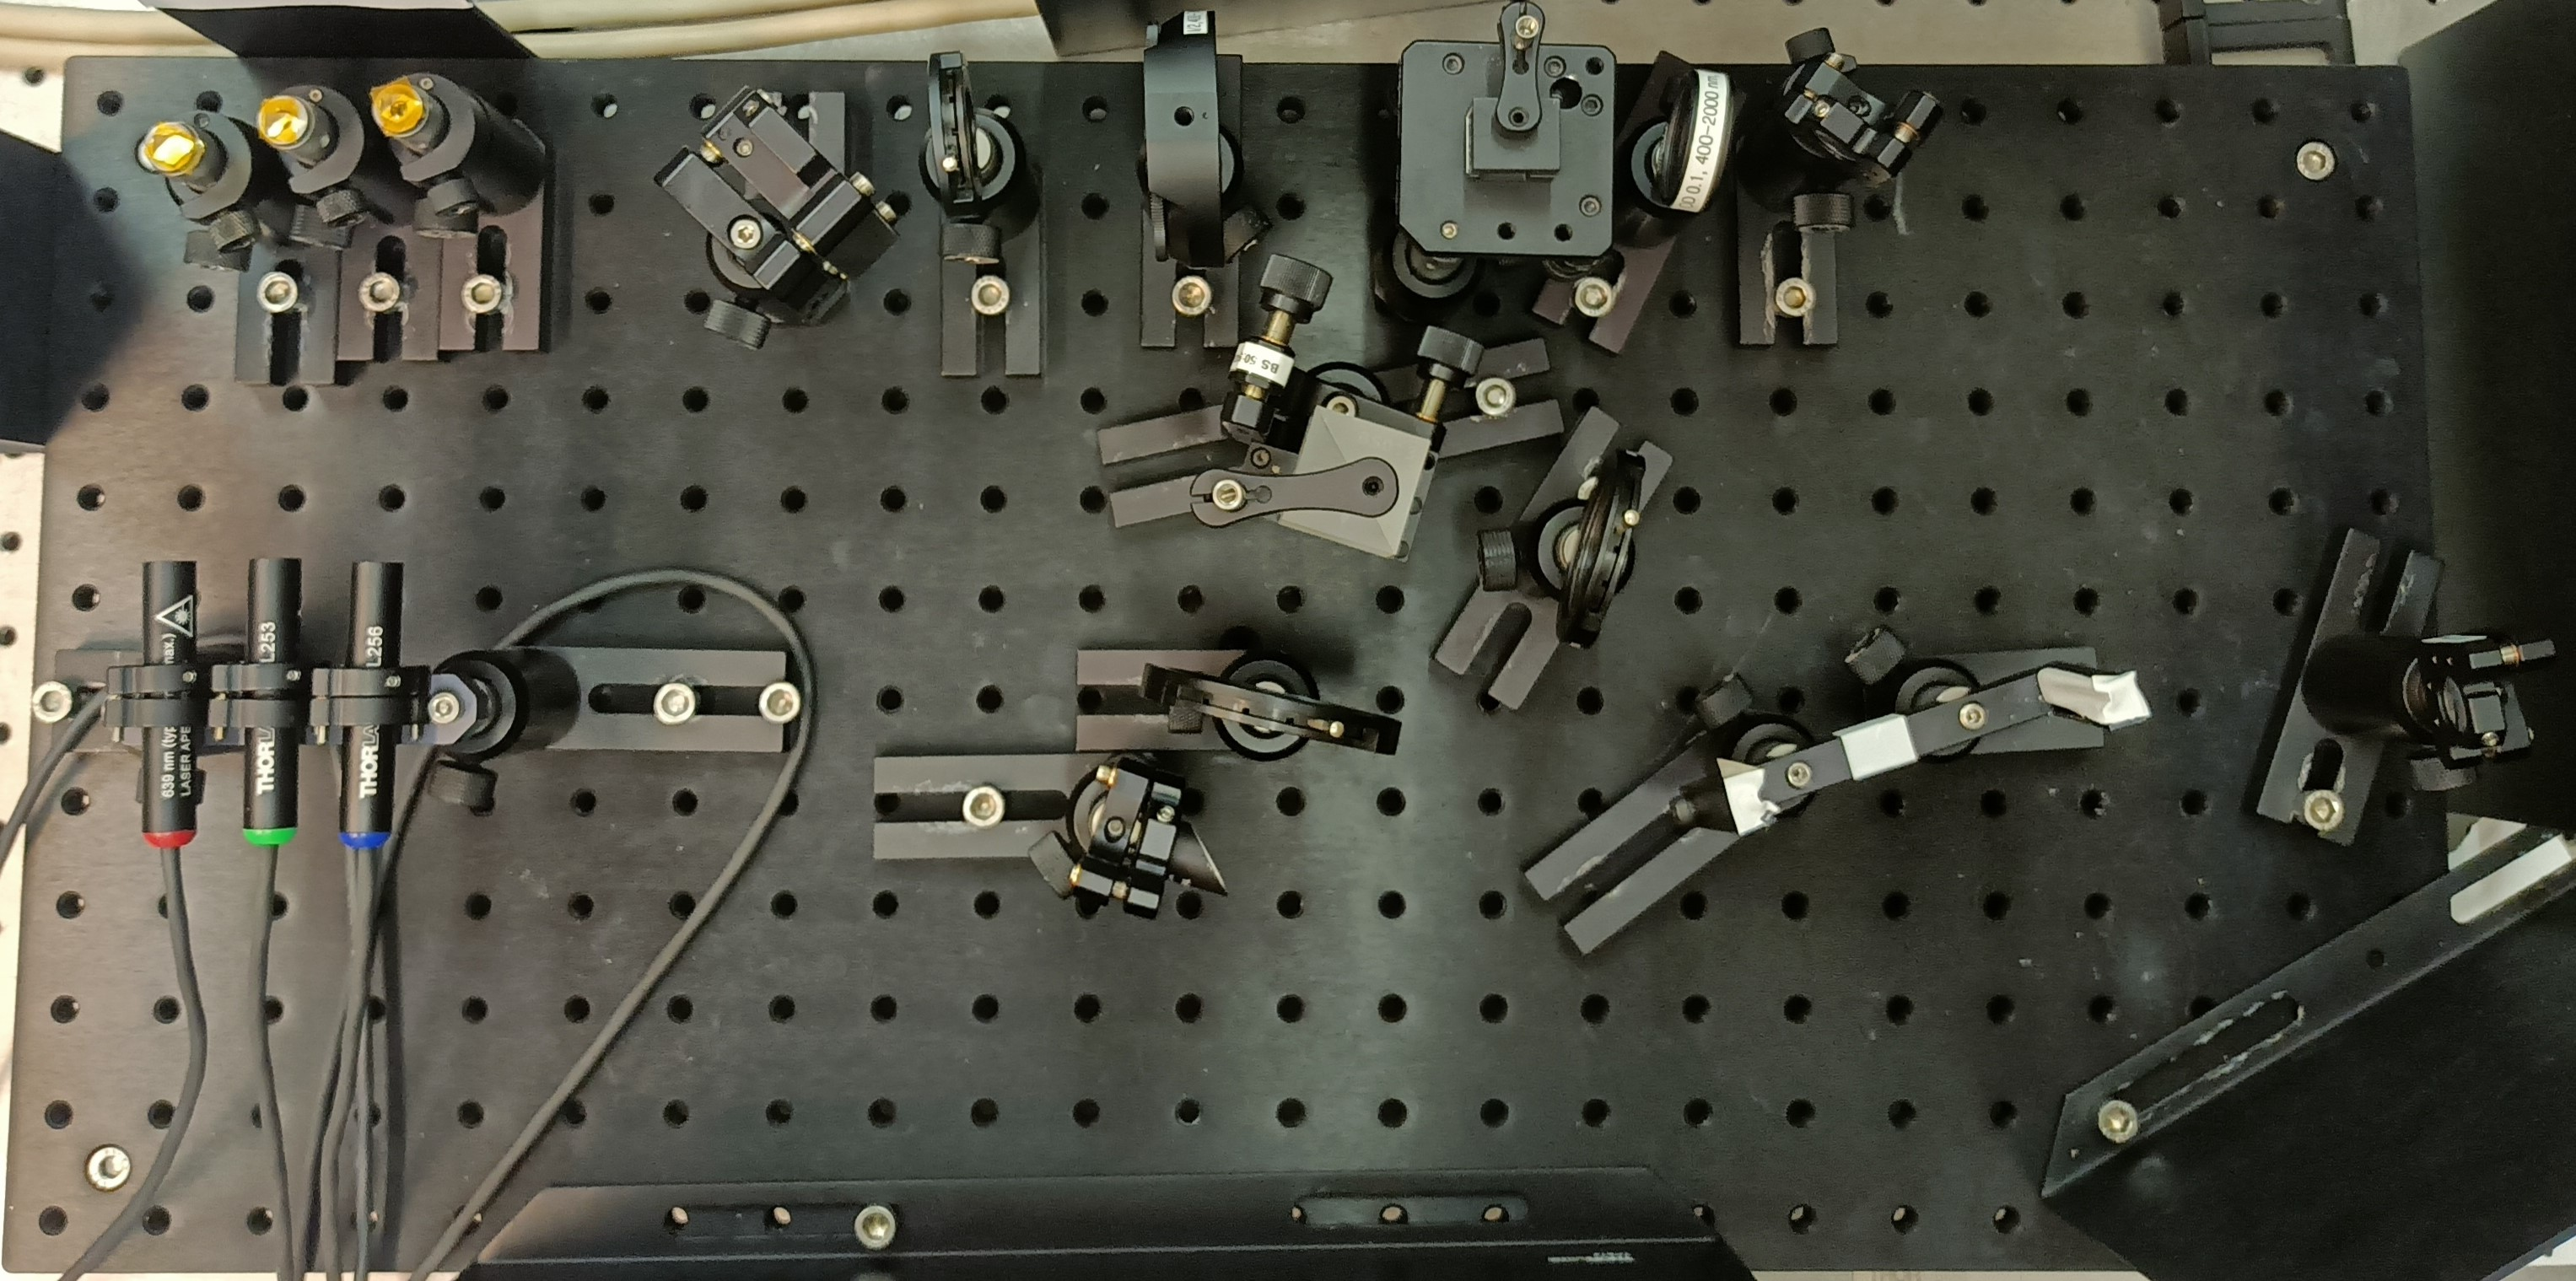
\includegraphics[width=\linewidth]{../img/nove-usporadani-shora.jpg}
    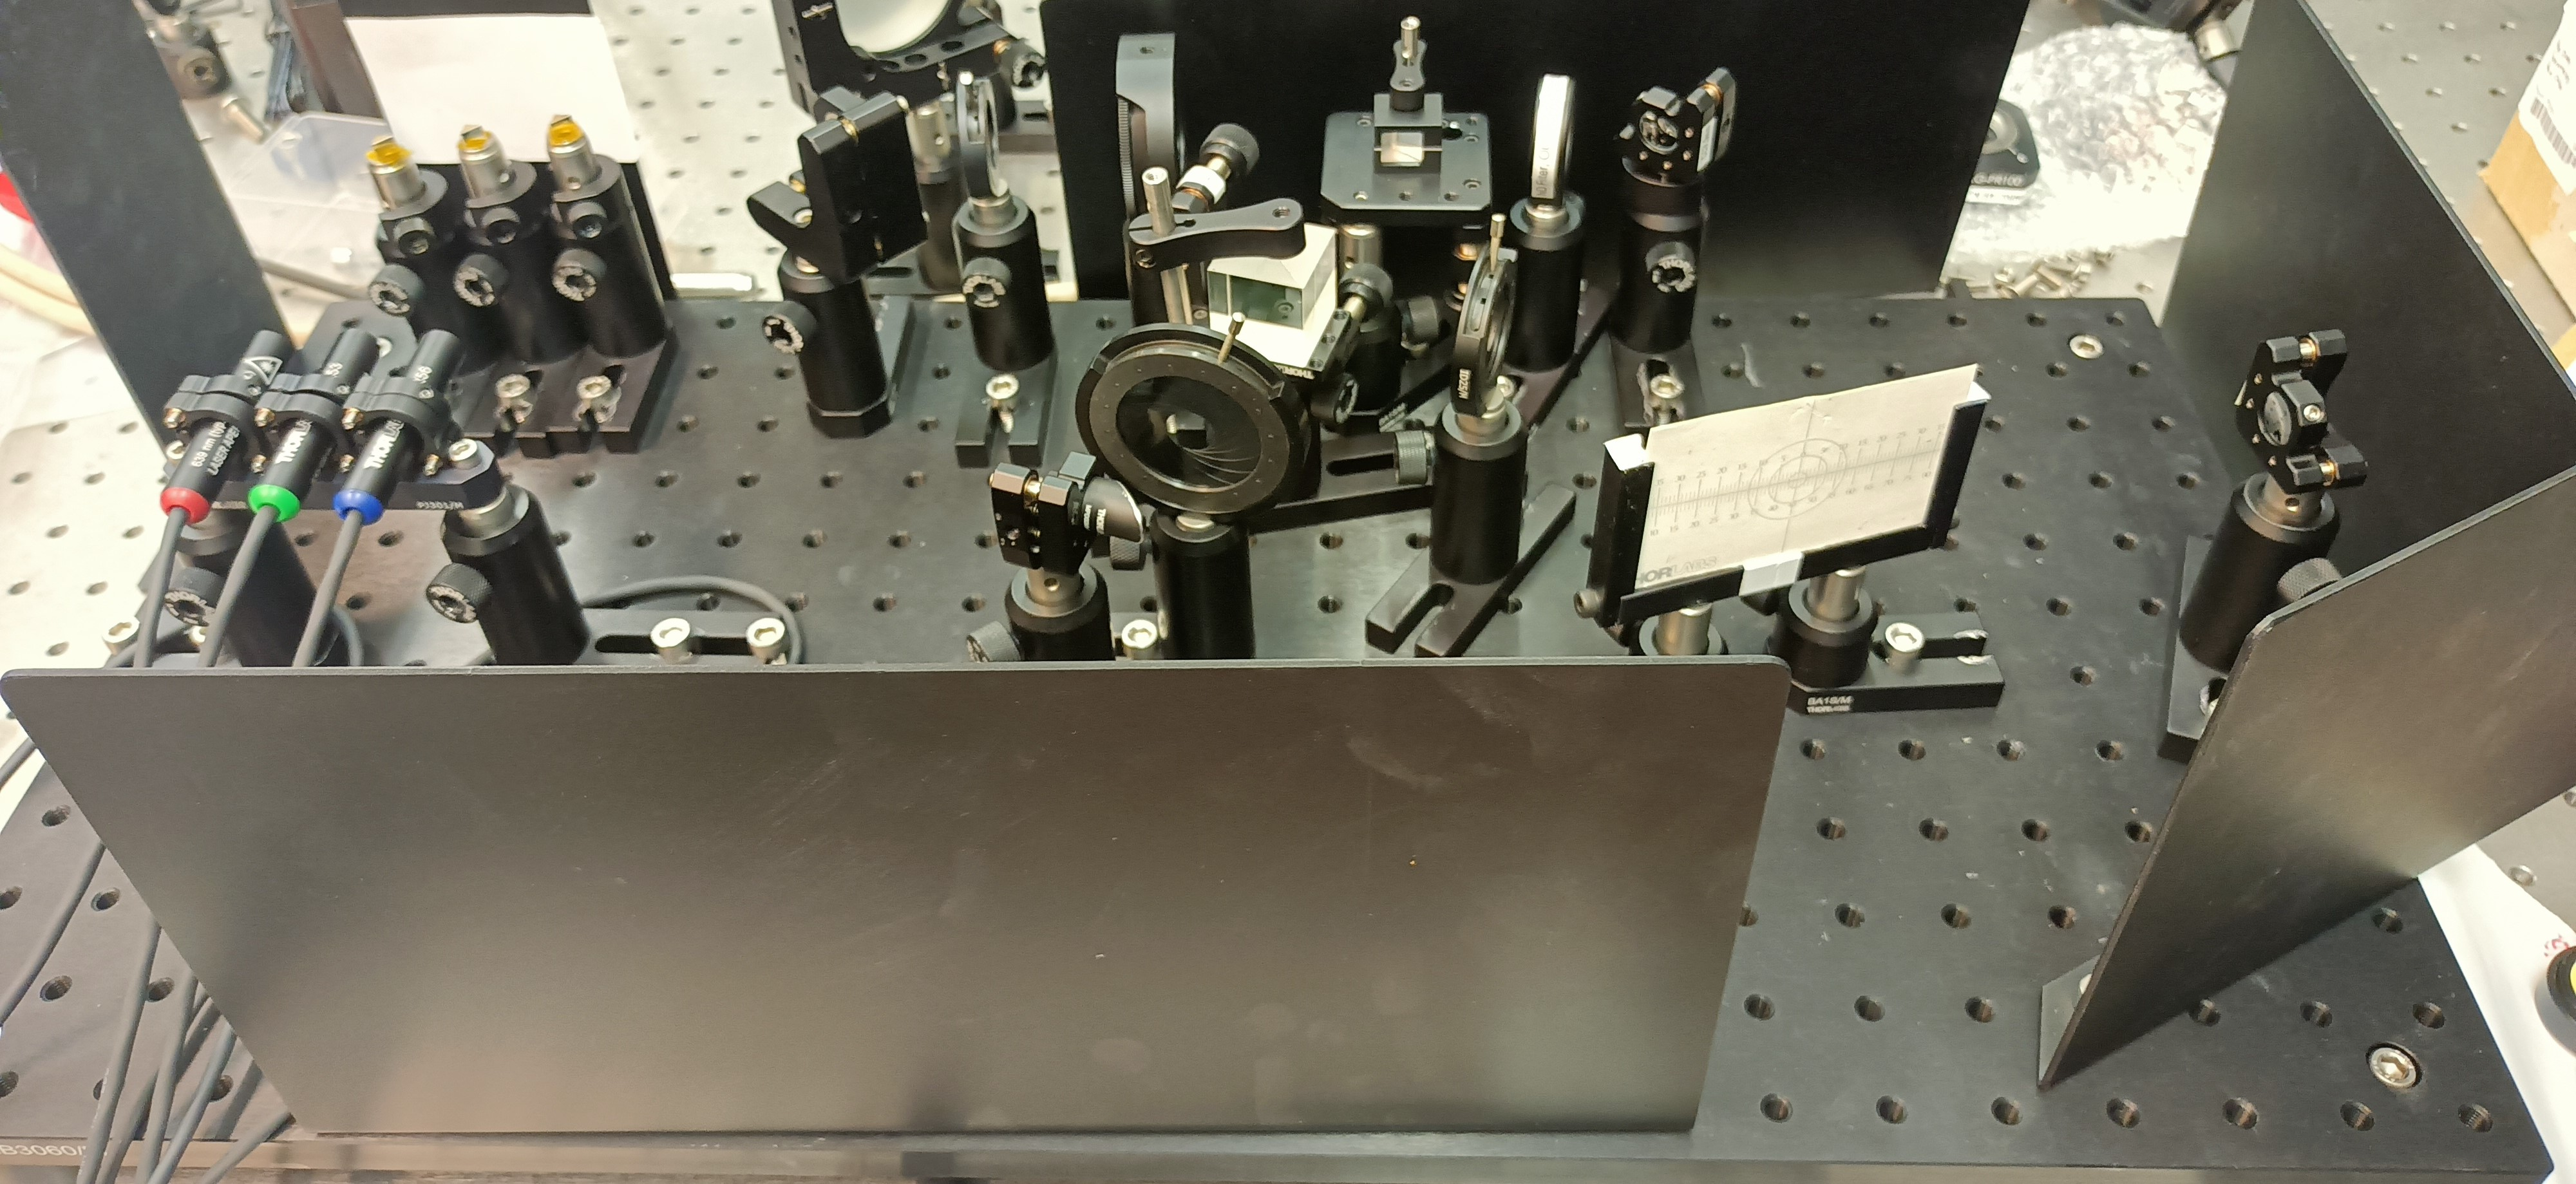
\includegraphics[width=\linewidth]{../img/nove-usporadani-uhel.jpg}
    \caption{Finální verze nového experimentálního uspořádání}
    \label{img:nove-usporadani}
\end{figure}

Obrázek experimentálního uspořádání \ref{img:nove-usporadani-popis} bez popisků a z dalšího úhlu je na obrázku \ref{img:nove-usporadani}.

\begin{figure}
    \centering
    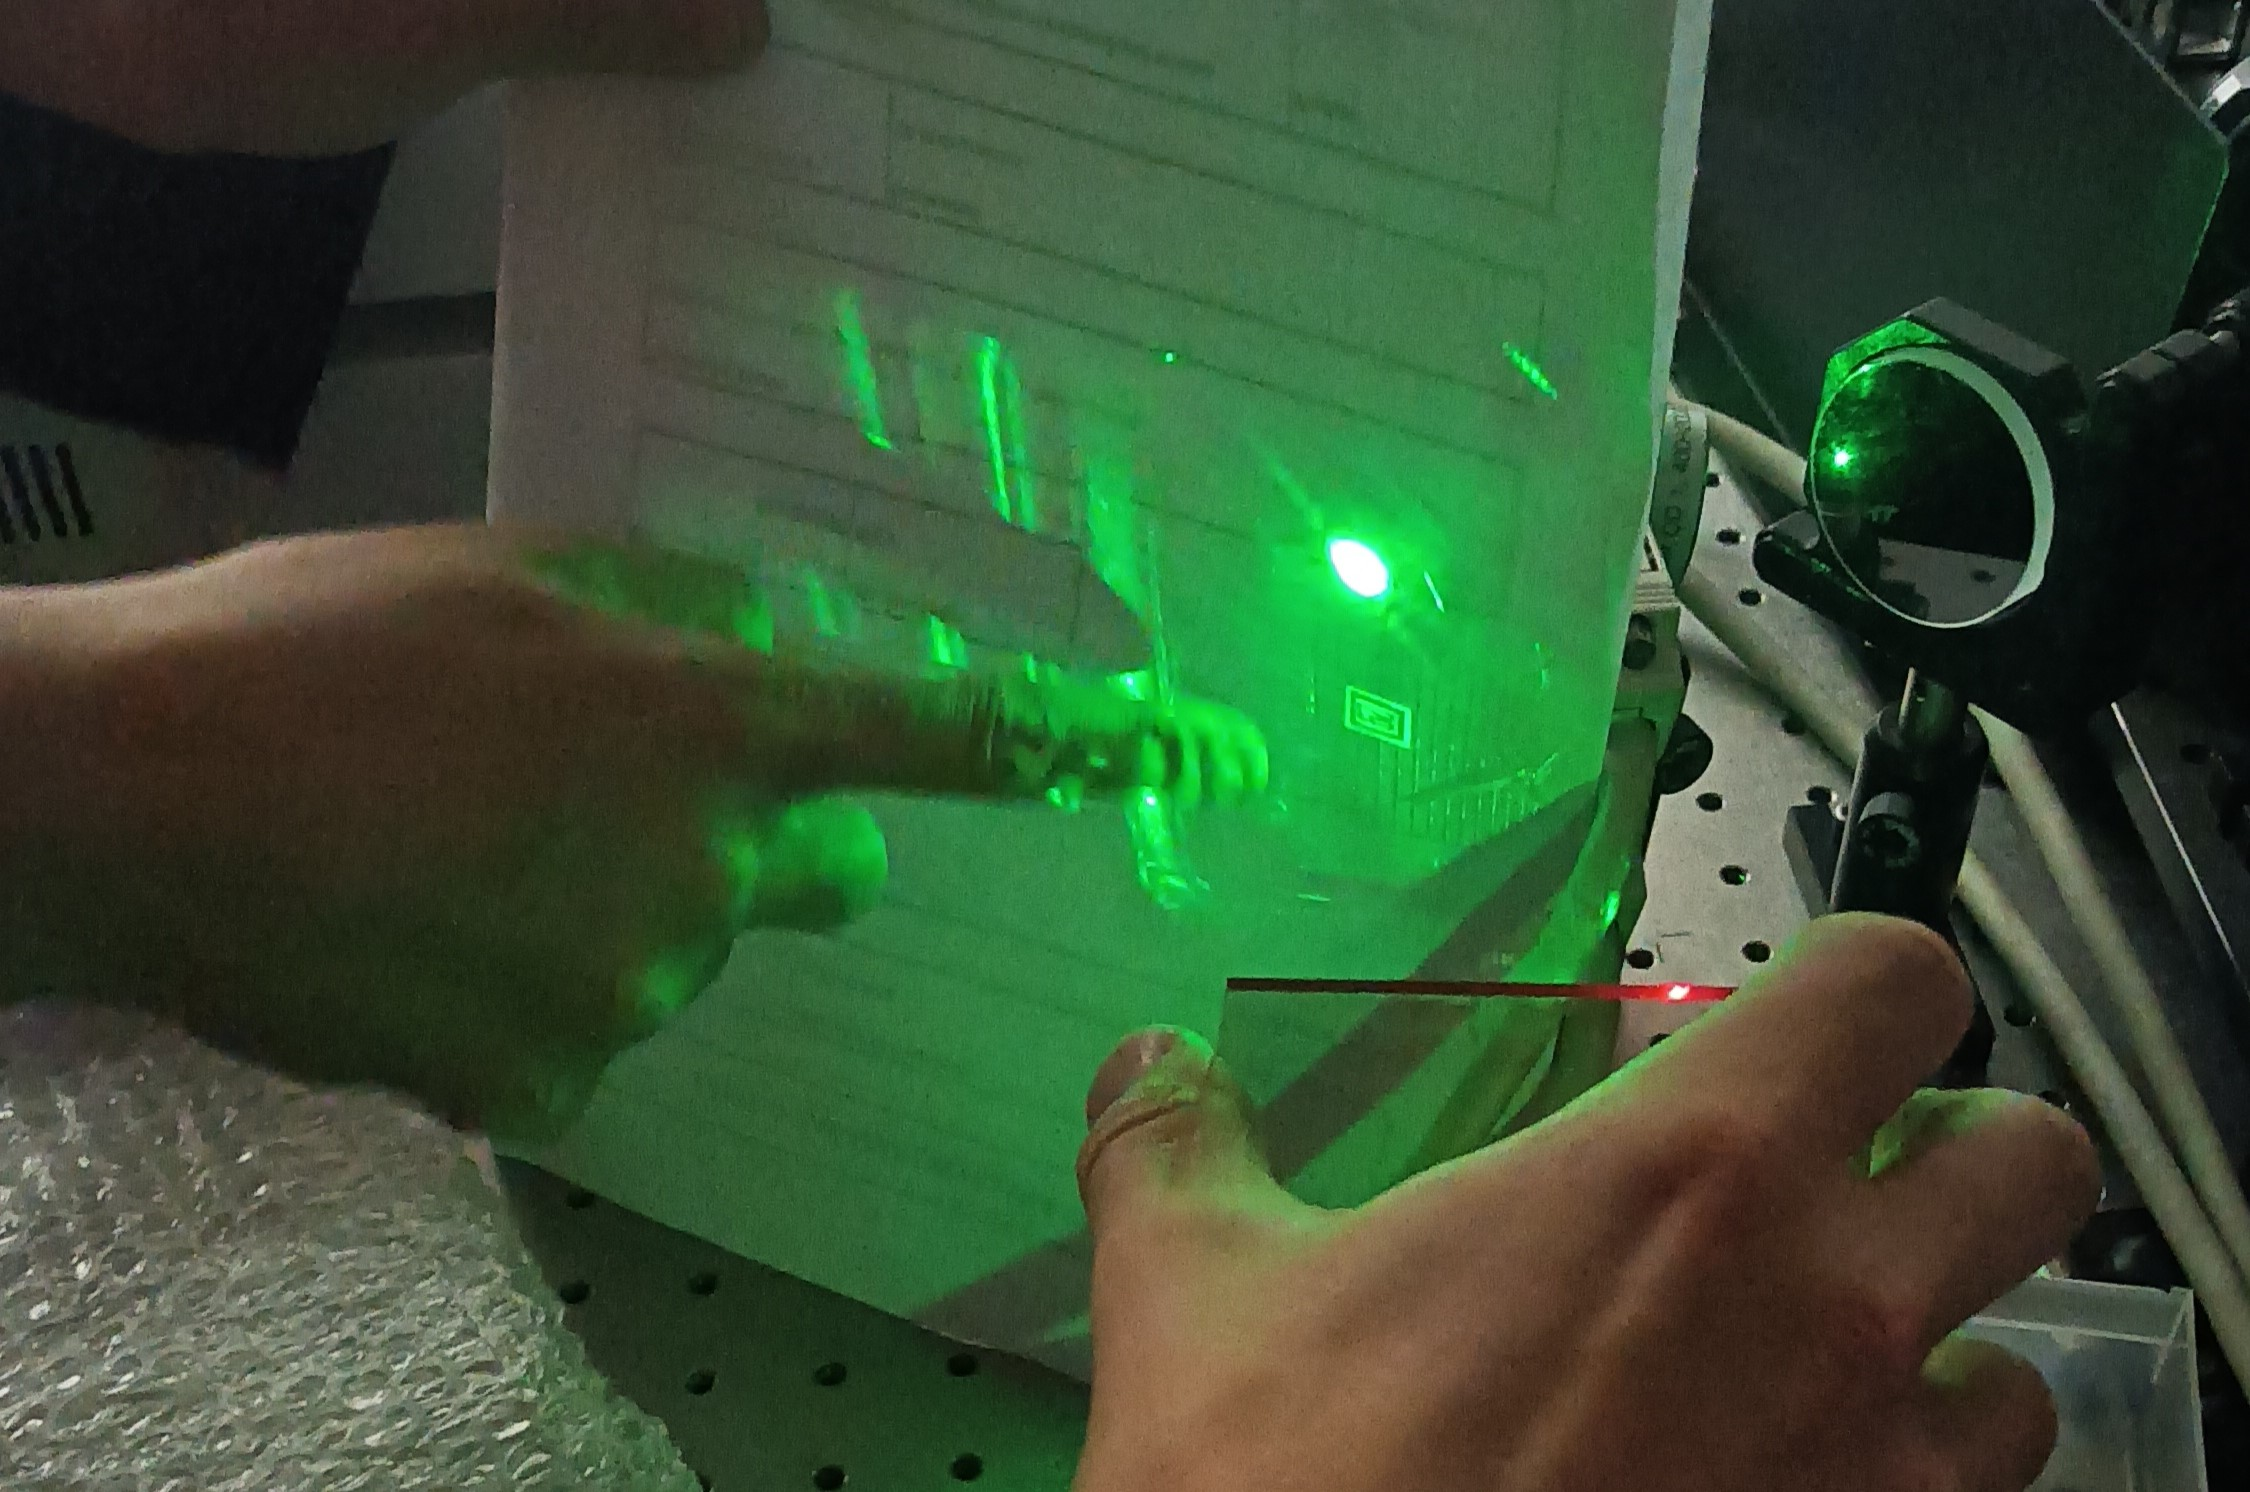
\includegraphics[width=\linewidth]{../img/hologram-t-projekce.jpg}
    \caption{Projekce monochromatického transmisního hologramu hodinek vytvořeného v novém uspořádání}
    \label{img:transmisni}
\end{figure}

\section{Holografické desky}
Nově jsou používány holografické desky výrobce \textbf{LitiHolo} \cite{litiholo}, které dokáží zaznamenávat hologramy v červené, zelené a modré barvě a jejich libovolné kombinaci, tedy lze vytvářet i bílé, resp. plně barevné, hologramy. Tyto desky jsou navíc samovyvolávací, není tedy potřeba žádná práce s chemikáliemi, pouze se doporučuje pro zlepšení kontrastu hologramu exponovanou desku dosvítit bílým světlem.

\begin{table}
    \caption{Vlnové délky a expoziční dávky pro expozici holografické desky (převzato z návodu dodaného s deskami)}
    \centering
    \begin{tabular}{|l|r|r|}
        \hline
        \textbf{barva} & \textbf{vlnová délka}\footnotemark[1] $\left[\text{nm}\right]$ & \textbf{expoziční dávka} $\left[\text{mJ.cm}^{-2}\right]$ \\
        \hline
        červená        & $635$                                                          & $20$                                                      \\
        zelená         & $532$                                                          & $30$                                                      \\
        modrá          & $450$                                                          & $80$                                                      \\
        \hline
    \end{tabular}
    \label{tbl:expozicni-davky}
\end{table}
\footnotetext[1]{Vlnová délka, na kterou je v dané barevné oblasti deska nejvíce citlivá.}

Tabulka \ref{tbl:expozicni-davky} ukazuje potřebné expoziční energie holografických desek. Jelikož pro lasery předpokládáme intenzitu $I$ konstantní a rozšiřujeme-li svazky tak, že jejich stopa v rovině holografické desky má plochu $S$, vypočteme expoziční dobu v sekundách
\begin{equation}
    t=\frac{\mathcal{E}\cdot S}{I}
    \label{eqn:expozicni-doba}
\end{equation}
z udané expoziční dávky $\mathcal{E}$. Máme-li intenzitu světla $I$ v miliwattech a plochu v $\text{cm}^2$, nemusíme ani provádět žádné převody jednotek.

\medskip

Při výrobě hologramů jsme vypozorovali, že na holografické desce vzniká při expozici viditelná mlhová stopa v místech, kam dopadá laserové světlo, a je-li intenzita příliš silná (např. při příliš dobrém odrazu v transmisním uspořádání), je fotocitlivá vrstva "`vypálena"' a stává se opět dobře průhlednou.

Dále je s holografickými deskami potřeba opatrnost při veškeré manipulaci, jelikož jsou zjevně vyrobeny jako fotocitlivá fólie nalepená na skleněné destičce, a při neopatrné manipulaci na hranách desky se začne fólie odlepovat. Drobná odlepení se neprojevila jako problém, fólie se snadno přilepí zpět, ale úplné odlepení by mohlo být problematické.

\section{Výroba hologramů\label{sec:vyroba-hologramu}}
Samotná výrba hologramů je velmi jednoduchá. V této sekci popíšeme i teorii obou typů hologramů, nicméně pro samotnou výrobu je potřeba jen zdroj napájení a rovný povrch v temné místnosti. Pro obě metody musíme na pozici (\texttt{5}) naměřit intenzitu světla $I$ a v rovině holografické desky (\texttt{10}) naměřit rozměry stopy laserových paprsků. Stopa bude mít tvar elipsy, stačí tedy naměřit délku hlavní polooosy $a$ a vedlejší poloosy $b$ a vzorcem
\begin{equation}
    S=\pi a b
\end{equation}
vypočítat plochu. Intenzitu $I$ a plochu stopy $S$ pak použijeme společně s expozičnámi dávkami z tabulky \ref{tbl:expozicni-davky} ve vzorci \eqref{eqn:expozicni-doba} k zísákní expoziční doby pro danou barvu.

Pro monochromatické hologramy toto znamená celkovou expoziční dobu, pro barevné hologramy toto udává dobu, po které je daný laser potřeba vypnout. Toto časování však za uživatele řeší software popsaný v kapitole \ref{cpt:software}.

\medskip

Z teoretického pohledu je výroba hologramů založená na interferenci referenční a objektové vlny ve fotocitlivém materiálu holografické desky. Realizace referenční a objektové vlny se v reflexním a transmisním uspořádání liší a je popsána v odpovídajících sekcích, nicméně mají společný princip. Vzniklé interferenční pole ve fotocitlivém materiálu iniciuje fotochemickou přeměnu, která permanentně zachytí rozložení intenzit interferujícího světla a vytvoří tak jakousi mřížku, jejímž následným osvětlením lze reprodukovat objektovou vlnu a tím vytvoři iluzi, že se objekt v daném místě skutečně nachází. Reprodukce se ale u obou metod také liší a je opět popsána v odpovídajících sekcích níže.

\subsection{Reflexní hologramy}
Reflexní hologramy jsou jednodušší na výrobu i pozorování, to ale za cenu toho, že vytvářejí pouze virtuální obraz -- tedy se zdá, že se objekt nachází za holografickou deskou, a konvexní povrchy se jeví jako konkávní a obráceně \cite{holography}. Hotové hologramy mohou být pozorovány v bílém světle pod úhlem, pod kterým byly exponovány, což je s malou destičkou v ruce jednoduché najít.

\medskip

V reflexním uspořádání je referenční a objektová vlna stejná, resp. referenční vlna se po průchodu holografickou deskou stává vlnou objektovou. Je tedy potřeba pouze jeden rozšířený svazek koherentního světla. Po průchodu holograficou deskou světlo dopadá na a odráží se od objektu a část odražená zpět na holografickou desku interferuje s přicházejícím světlem, čímž vzniká interferenční pole ve fotocitlivé vrstvě.

\medskip

Při exponování hologramů v reflexním uspořádáním nasměrujeme pomocí kombinace půlvlnové destičky (\texttt{4}) veškerou intenzitu do ramene přímo dopadajícího na holografickou desku a uzavřením irisových clonek (\texttt{c}) v druhém rameni odstíníme případné zbytkové světlo. Objekt umístíme na podstavci na plochu (\texttt{11}) tak, aby se pokud možno dotýkal holografické desky -- tím jsou deska a objekt spojeny tak, že vibrují společně, a vibrace tedy nepůsobí problémy s kvalitou hologramu.

\subsection{Transmisní hologramy}
Hologramy transmisní vyžadují vyšší stabilitu i expoziční dobu pro vytvoření a k jejich pozorování je nutné laserové světlo ideálně takové, kterým byly vyrobeny. Za tuto cenu ovšem získáme možnost pozorovat reálný obraz \cite{holography}, který můžeme promítnout tak, jak je ukázáno na obrázku \ref{img:transmisni}. Tato projekce se provádí bodovým laserovým světlem, roztažením laserového svazku pak lze měnit velikost obrazu a vzdálenost, ve které se jeví jako ostrý. Tento reálný obraz lze také použít dále pro proces \textit{sekundární holografie}, tedy vytvoření hologramu z hologramu namísto objektu \cite{holography}, neboli kopírování.

U transmisních hologramů je možné pozorovat i virtuální obraz \cite{holography}, a to nejlépe umístěním vyvolané holografické desky zpět do držáku v experimentálním uspořádání. Tím zaručíme stejné osvětlující světlo i úhel a tedy nejvyšší kvalitu hologramu. Zde však laserové světlo musí holografickou deskou projít, a tedy svítí do podobného prostoru, ze kterého je virtuální obraz pozorovatelný. Pozorovatel tak musí být opatrný, aby se nepodíval přímo do laserového svazku, a intenzita referenční vlny použitá pro rekonstrukci tohoto virtuálního obrazu musí být bezpečně nízká.

\medskip

V tomto uspořádání jsou referenční a objektová vlna separátní: Referenční vlna dopadá přímo na holografickou desku, zatímco objektová vlna musí dopadnout na objekt až za deskou a odrazit se na ni od objektu. Referenční a objektová vlna nemají stejnou intenzitu, nejvhodnější (z hlediska kvality hologramu i výpočtu poměru intenzit) je nasměrovat $20\,\%$ intenzity do referenční vlny a $80\,\%$ do objektové vlny \cite{projekt}.

Je možné také objektovou vlnu rozdělit na více a osvětlovat objekt z více úhlů. To pak dává více úhlů, ze kterých lze hologram pozorovat (odpovídají okolí úhlů objektových vln). V našem uspořádání byla objektová vlna rozdělena na dvě, ty byly navíc nastaveny tak, aby každá osvětlovala v trochu jiné hloubce. To by mělo vést k dobré pozorovatelnosti pod více úhly a lepšímu zachycení hloubky objektů.

\medskip

Při exponeování hologramů v transmisním uspořádání za pomoci měřiče intenzity a kombinace půlvlnové destičky (\texttt{4}) nasměrujeme intenzitu laserového světla do větve referenční vlny a větve objektové vlny ve výše uvedeném poměru. Irisové clonky (\texttt{c}) otevřeme tak, aby propouštěly primární svazky, ale stínily různé násobné odrazy a interferenční pole, vzniklé např. na děliči (\texttt{7}). Objekt umístíme na podstavci na plochu (\texttt{11}) tak, aby byl co nejlépe osvětlen objektovou vlnou. Zde není možné, aby se dotýkal holografické desky, transmisní hologramy tedy budou náchylnější na vibrace.

\section{Náměty na zlepšení}
Uvádíme zde seznam námětů, na které jsme při experimentech narazili a které by bylo do budoucna přínosné zlepšit, ale nebyly nezbytné pro úspěšné sestavení experimentálního uspořádání. Jsou zde uvedeny za účelem postupného vylepšování, naskytne-li se příležitost.

\subsection*{Fluorescenční značky}
Holografické desky musejí být před samotnou expozicí uchovávány v co největší tmě, což také vyžaduje, aby byly vyndavány z balení a umisťovány do držáku v temné místnosti. Orientace po hmatu je sice možná, ale je nepraktická a hrozí rozladění aparatury či znečištění povrchu citlivých optických komponent dotykem.

Při pokusech jsme na optickém stole měli připravený měřák intenzity, jehož sonda je po obvodu vyrobena z fluorescenčního materiálu. Ukázalo se, že tento prvek je výborným orientačním bodem pro navigaci v temné místnosti a zároveň je intenzita světla vycházející z tohoto prvku velmi nízká.

Umístěním fluorescenčních značek např. na vnější stranu stínítek by byla značně zjednodušena orientace v temné místnosti a neměly by negativně ovlivnit kvalitu hologramu.

\subsection*{Uchycení zrcátek}
Malá trojúhelníková zrcátka (\texttt{2}) v obrázku \ref{img:nove-usporadani-popis} jsou upevněna relativně dočasně na tyčkách pomocí oboustranné lepící pásky. Jelikož byla zrcátka lepena ručně a manipulace s nimi není jednoduchá, nejsou všechna zrcátka nalepena stejně a jsou přilepena pod různým úhlem, který musí být kompenzován uchycením laseru.

V laboratoři je k dispozici "`beam combiner,"' který je určen přesně pro účel přiblížení laserových svazků, má ale špatné rozměry. Pro méně robustní řešení by bylo možné ponechat stávající umístění zrcátek a použít úchyty zrcátek z "`beam combineru,"' našel-li by se způsob převodu M3 a M4 závitů, ideálním řešením by však bylo sehnat či vyrobit "`beam combiner"' s vhodnou roztečí zrcátek.

\subsection*{Modrý laser}
V sekci \ref{sec:usporadani} uvádíme, že modrý laser má nevhodnou vlnovou délku $402{,}1\,\text{nm}$, která nejenže neexponuje holograficou desku dobře, ale navíc na ní ani správně nefungují některé komponenty. Zrcátko (\texttt{2}) a půlvlnová destička (\texttt{4}) z obrázku \ref{img:nove-usporadani-popis} se ukázaly jako obzvláště problematické.

Laser má na svém výstupu intenzitu světla cca. $4{,}6\,\text{mW}$. Po odrazu na zrcátku ale pokračuje dále do uspořádání pouze přibližně $3{,}6\,\text{mW}$ a dále za půlvlnovou destičkou jsme naměřili již jen asi $2{,}6\,\text{mW}$. To je intezita již příliš nízká pro praktické využití, jelikož dle tabulky \ref{tbl:expozicni-davky} vyžaduje modrá barva nejvyšší expoziční dávku. To vedlo na expoziční dobu kolem $40\,\text{min}$, při které se již ztrácí stabilita laserového výstupu i vibrací aparatury.

Při expozici všemi třemi barvami laseru jsme byli schopni pozorovat modré a bílé oblasti hologramu, tedy se modrá složka holografické desky tímto světlem exponovala, nicméně při expozici pouze tímto modrým laserem jsme na desce žádný hologram nenalezli. Pro účely barevené holografie tedy bude postačující nalézt zrcátko a půlvlnovou destičku, které budou fungovat dobře se všemi třemi barvami laserů, aby se snížila expoziční doba, ale obecně by bylo vhodné modrý laser nahradit jiným, který bude mít vlnovou délku bližší $450\,\text{nm}$ doporučeným výrobcem holografických desek.

\subsection*{Držák holografické desky}
Současný držák holografické desky (\texttt{10}) je vyroben z různých dílů optické "`stavebnice"' a jeví se jako velmi praktický. Disponuje pozicí na umístěhí holografické desky i kalibrační papírové kartičky, jak je vidět na obrázku \ref{img:nove-usporadani} dole.

Pozice pro umístění holografické desky je ale momentálně závislá na elektrikářské lepící pásce, která ačkoli díky své pružnosti velmi dobře drží holografickou desku, její opotřebení je nevyhnutelné. Do budoucna tedy bude muset být páska vyměňována, nebo bude potřeba vytvořit gumové vložky do drážek držáku, které zajistí pevné uchycení desky s trvalejší životností.

\chapter{Elektronická část\label{cpt:elektronika}}
\begin{center}
    Tato kapitula stručně popisuje elektronický obvod a komponenty použité k napájení a řízení laserů a vizuální a akustickou indikaci pro uživatele.
\end{center}
\begin{figure}[!ht]
    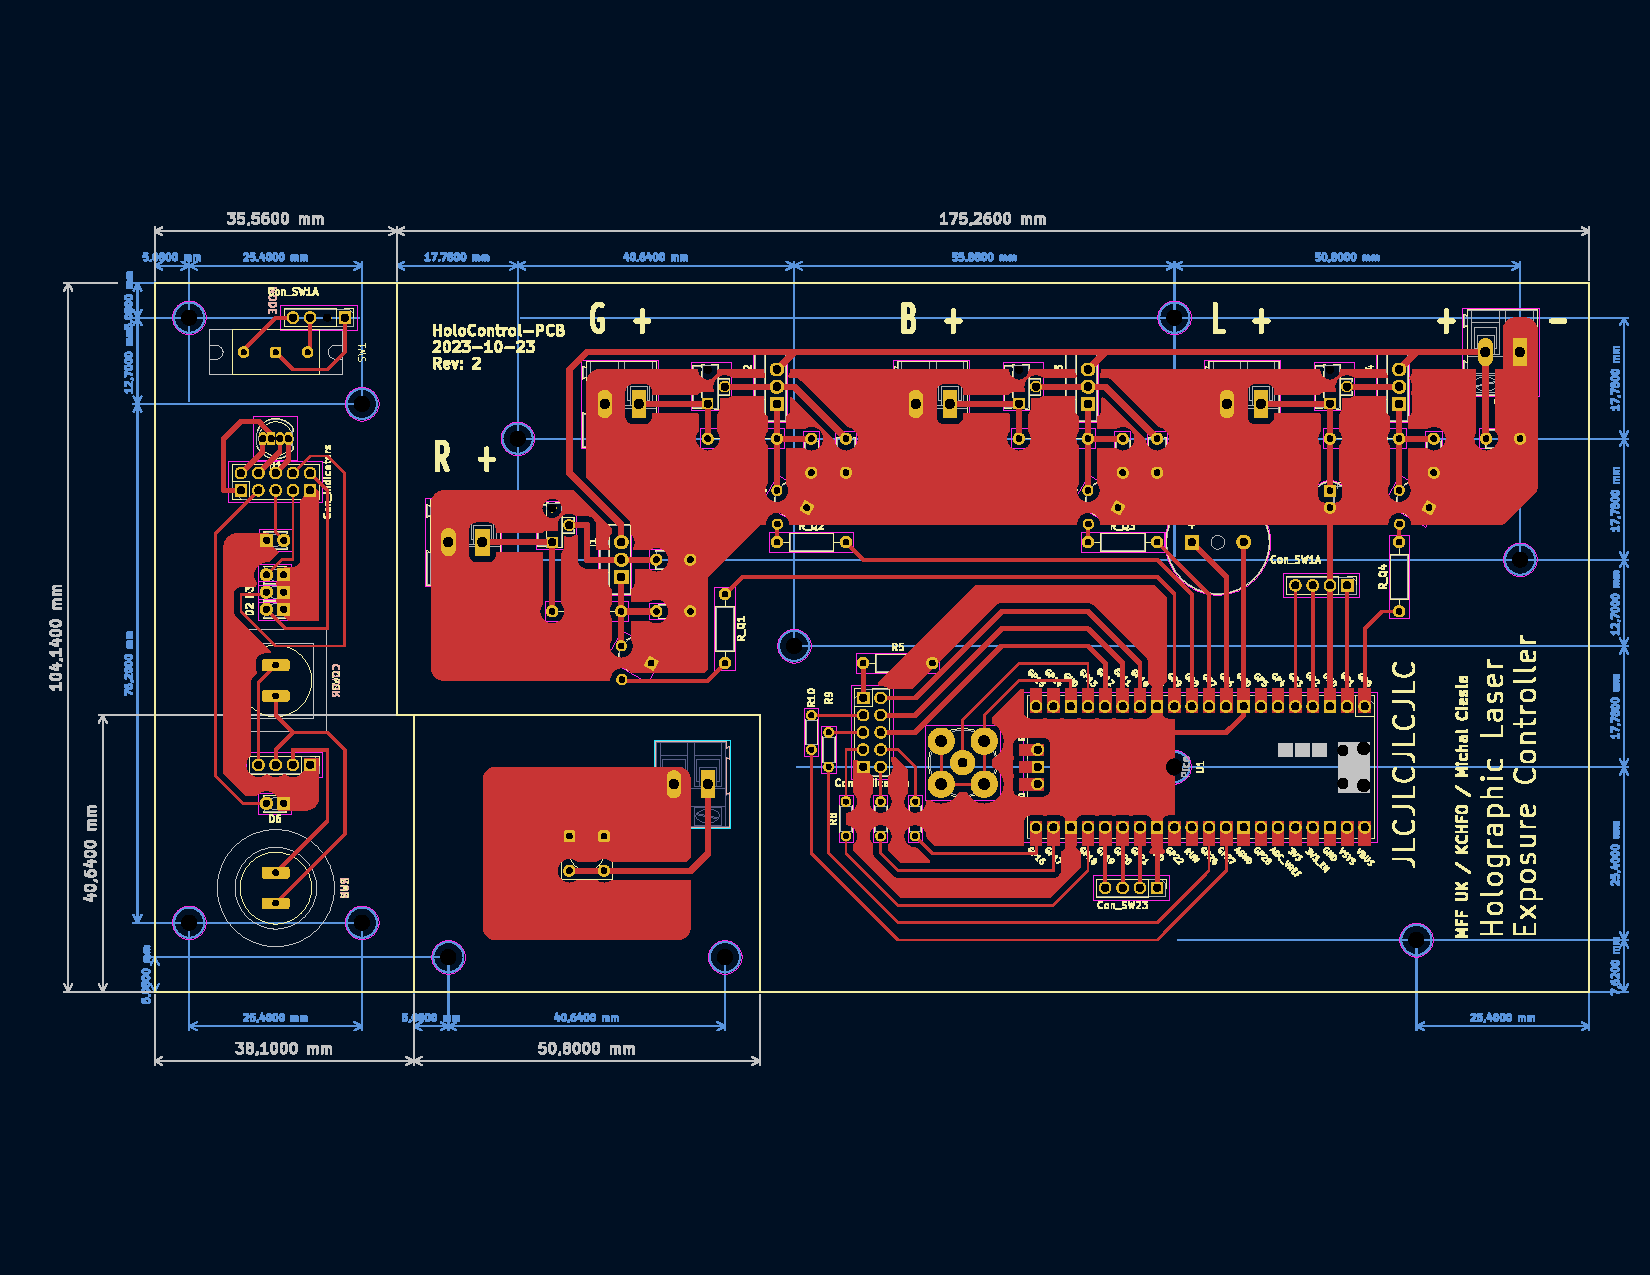
\includegraphics[width=\linewidth]{../../HoloControl-PCB/holo-controller-pcb.pdf}
    \caption{Schéma řídícího elektronického obvodu}
    \label{img:schema}
\end{figure}

Elektronický obvod je postaven kolem řídícího mikrokontroleru \textbf{Raspberry Pi Pico}, který digitálními signály na různých svých výstupech zprostředkovává následující funkce:
\begin{itemize}
    \item spínání laserů dle nastaveného časování,
    \item spínání dosvětlovací LED,
    \item ovládání externího laseru pomocí TTL signálu,
    \item akustickou indikaci zahájení a dokončení expozice v automatickém režimu a
    \item světelnoou indikaci právě rozsvícených laserů v manuálním režimu.
\end{itemize}
Jako vstupy používá přepínač režimů (manuální nebo automatický), dvojici tlačítek pro fyzickou interakci a USB port pro sériovou komunikaci. Manuální režim slouží pro testování a měření intenzit laserového světla, v automatickém režimu mikrokontroler spíná lasery po nastavené časy (udržuje každý laser rozsvícený po nastavenou dobu, aby bylo dosaženo potřebné expoziční dávky). Další klíčovou rolí elektronického obvodu je udržování konstantního výkonu laserů.

\medskip

Na hlavní desce plošných spojů je umístěn mikrokontroler, moduly pro napájení a spínání laserů (oblast \textit{Lasers} v obrázku \ref{img:schema}, mimo laserových diod) a dosvětlovací LED (oblast \textit{Finishing LED}, mimo samotné LED), BNC konektor pro výstup na externí laser (oblast \textit{TTL}) a piezoelektrický bzučák pro akustickou indikaci. Lasery jsou připojeny pomocí oddělených svorkovnic. Ovládací a indikační prvky a dosvětlovací LED jsou umístěny na vlastních deskách plošných spojů a připojují se odlišenými konektory.

\section{Ovládací panel}
Ovládací panel tvoří fyzickou interakční plochu pro uživatele a jemu příslušející elektronika je umístěna na separátní desce plošných spojů. Na ovládacím panelů se nachází
\begin{itemize}
    \item trojice LED v barvách odpovídajících barvám laserů, které v manuálním režimu indikují sepnutí napájení laserů,
    \item teplá bílá LED, která v manuálním režimu indikuje signál \texttt{HI} na TTL spojení s externím laserem,
    \item studená bílá LED, která v manuálním režimu indikuje rozsvícení dosvětlovací LED,
    \item RGB LED, která svou barvou indikuje mauální režim (modře), automatický režim (zeleně) nebo chybový stav (červeně),
    \item přepínač režimů (manuální nebo automatický),
    \item tlačítko, které v manuálním režimu cyklicky přepíná mezi lasery a v automatickém režimu spouští, pozastavuje či ukončuje expozici, a
    \item tlačítko, které v manuálním režimu zapíná a vypíná dosvětlovací LED a v automatickém režimu zhasíná RGB LED.
\end{itemize}
Ve schématu na obrázku \ref{img:schema} toto odpovídá oblastem \textit{Status}, \textit{Manual Color Select} a \textit{Mode Select}.

\section{Napájení laserů}
Lasery jsou napájeny digitálně spínanými obvody pro stabilizaci proudu postavenými na napěťových regulátorech \textbf{LM317T}. V oblasti \textit{Lasers} na obrázku \ref{img:schema} jsou umístěny tři paralelní moduly, které při napájení báze tranzistorů \texttt{Q1}-\texttt{Q3} nepouštějí do laserů žádný proud, resp. ne dostatečný pro jejich rozsvícení. Samotné lasery vyznačené ve schématu pak na desce plošných spojů reprezentují oddělené dvoupólové svorkovnice, do kterých se napájecí kabely laserů zapojí.

Obvody pro stabilizaci proudu poskytují stabilní napájení laserů a také reagují na jejich zahřívání. Stabilizace proudu je dobrým kompromisem pro nenáročnou a relativně precizní stabilizaci výstupního výkonu laserů. Díky trimrům \texttt{R1}-\texttt{R3} je také možné pro každý laser nezávisle nastavit protékající proud.

Zapojení modulů pro digitálně spínatelnou stabilizaci proudu je převzato z \cite{system}.

\section{Dosvětlovací LED}
Dosvětlovací LED je napájena obvodem z velké míry totožným s obvodem pro napájení laserů. Jediným rozdílem je zapojení a kapacita kondenzátoru \texttt{C\_I4} (viz obrázek \ref{img:schema}). Tento kondenzátor je zapojen přímo na LED a jeho řádově vyšší kapacita způsobuje pomalé a plynulé zhasínání LED, což je pro zvolený typ LED šetrnější.

Pro dosvětlování byla zvolena tzv. \textit{Superflux LED}, která má na své malé rozměry a nízký proud ohromný světelný tok. Tato LED je umístěna na malé desce plošných spojů společně jen s konektorem, jelikož bude v experimentálním uspořádání umístěna před držákem holografické desky (mezi pozicemi (\texttt{5}) a (\texttt{10}) na obrázku \ref{img:nove-usporadani-popis}) v nakloněné poloze. Minimální počet součástek snižuje náchylnost na poškození při manipulaci.

\section{Externí laser}
Jelikož očekáváme připojování externího laseru, který je napájen vlastní řídící jednotkou, poskytuje elektronický obvod také výstup ve formě BNC koaxiálního konektoru, na který je přiváděn TTL signál\footnote{Úroveň \texttt{HI} je u \textbf{Raspberry Pi Pico} pouze $3{,}6\,\text{V}$, nikoliv pro TTL typických $5\,\text{V}$, to je nicméně dostatečně nad hranicí mezi \texttt{HI} a \texttt{LO} a signál bude přijímačem interpretován správně.} pro vyžádání zapnutí či vypnutí externího laseru. Řídící jednotky laserů se liší svým ovládáním, typicky ale předpokládáme situaci, že jako stav laseru budou zrcadlit signál na svém TTL vstupu, případně jej invertovat. Pro konkrétní řídící jedmotky je vždy možné pozměnit kód mikrokontroleru, v případě častého střídání řídících jednotek je možné kód mikrokontroleru rozšířit o instrukce pro nastavení typu TTL komunikace.


\vfill
\noindent
\textit{Kompletní technická dokumentace elektronického obvodu bude zpracována a předána pracovišti po formálním ukončení projektu.}
\chapter{Softwarová část\label{cpt:software}}
\begin{center}
    Tato kapitula přehledově vysvětluje ovládání celého systému jak z pohledu mikrokontroleru, tak z pohledu uživatele jak pomocí přímé sériové komunikace, tak pomocí uživatelského grafického rozhraní.
\end{center}

% TODO: Úvodní odstavce

\section{Řídící mikrokontroler}
Kód pro mikrokontroler \textbf{Raspberry Pi Pico} byl napsán v jazyce C s pomocí knihoven poskytovaných v rámci \textbf{Raspberry Pi Pico SDK}. Má za úkol zpracovávat vstupy z fyzických ovládacích prvků i sériového/USB portu, zajišťovat akustickou a vizuální indikaci, spínat napájecí obvody laserů a, klíčově, časovat dobu zapnutí jednotlivých laserů.

Mikrokontroler může běžet ve dvou režimech: manuálním a automatickém. Manuální režim slouží pro testování a měření intenzity laserového světla a je detailněji popsán v předchozí kapitole \ref{cpt:elektronika}. Automatický režim slouží pro expozici hologramů po předem definovanou dobu.

\subsection{Časování}
Mikrokontroler prochází hlavní programovou smyčkou s uměle sníženou periodou $1\,\text{ms}$, aby tato smyčka byla co nejvíce časově stabilní i při zahřátí nebo stárnutí mikrokontroleru, které mohou lehce změnit základní takt procesoru. To zároveň umožňuje velmi jednoduché měření času expozice v milisekundách, které se změní na prosté počítání cyklů hlacní smyčky.

Milisekundy jsou dostatečně, ba až zbytečně, jemným krokem pro účely holografie, kde se v případě tohoto experimentálního uspořádání pracuje s expozičními dobami v řádu desítek sekund až desítek minut. Pro případy velmi výkonných externích laserů by se však eventuelně milisekundová přesnost mohla hodit.

\medskip

Pomocí sériové komunikace lze mikrokontroleru nastavit
\begin{itemize}
    \item dobu čekání před zahájením expozice (čas pro uživatele, aby opustil laboratoř),
    \item dobu expozice červeným laserem,
    \item dobu expozice zeleným laserem,
    \item dobu expozice modrým laserem,
    \item dobu expozice externím laserem a
    \item čas, po který bude zapnuta dosvětlovací LED.
\end{itemize}
Předpokládá se, že uživatel z naměřeného světelného výkonu laserů a potřebné expoziční dávky v dané oblasti spektra vypočte expoziční dobu ze vzorce \eqref{eqn:expozicni-doba} a na mikrokontroleru ji nastaví. Doba čekání a doba dosvětlování mohou být zvoleny arbitrárně dle potřeby.

Po spuštění expozice, ať už fyzicky tlačítkem nebo počítačově, se spustí odpočet čekání, což je také indikováno akusticky. Po vypršení doby čekání jsou rozsvíceny všechny lasery s nenulovou expoziční dobou, což je opět doprovázeno akustickou signálizací. Program odpočítává cykly hlavní smyčky a jakmile je dosaženo nastavené expoziční doby některého z laserů, je tento laser vypnut. Jakmile je vypnut poslední laser, je dokončení expozice opět oznámeno akusticky a je-li nastavena nenulová doba dosvětlování, je zapnuta dosvětlovací LED. Po dosažení i jejího nastaveného času je zhasnuta a úplné dokončení je doprovozeno posledním zvukovým signálem.

\subsection{Komunikace}
\textbf{Raspberry Pi Pico} je vybaveno micro-USB portem pro napájení a sériovou komunikaci. Obě funkce tohoto portu využíváme.

Pro nastavování dob expozice a případně také nahrazení interakce s fyzickými tlačítky byl pro komunikaci s mikrokontrolerem navržen primitivní protokol se čtyřbajtovými instrukcemi. Instrukce nejsou člověku srozumitelné a nelze je interpretovat textově, jsou však velmi rychlé na zpracování, což je pro časovou stabilitu hlavní programové smyčky zásádní.

\medskip

Ve zkratce se každá instrukce skládá z příkazu, který je reprezentován prvním bajtem, a dat, pro která jsou určeny zbylé tři bajty. Data mohou být některými příkazy nevyužita, některé příkazy je využívají pro nastavení stavu zapnuto/vypnuto, a příkazy pro nastavení časování je využívájí právě pro nastavení času. Časy se nastavují v milisekundách, pro které 3 bajty, tedy 24 bitů, dávají maximální nastavitelnou dobu expozice/čekání/dosvětlování $2^{24}\,\text{ms}=16\,777\,216\,\text{ms}\approx4{,}7\,\text{h}$. Podrobnější popis instrukcí včetně jejich seznamu se nachází v příloze \ref{cpt:appendix}.

\section{Uživatelské ovládací prostředí}
Ovládání časování pomocí číselných (resp. šestnáctkových, viz příloha \ref{cpt:appendix}) instrukcí ze sériového terminálu je uživatelsky značně nepřívětivé, obzvláště pak pro případ využití na propagačních akcích. Proto k projektu bylo vytvořeno také grafické uživatelské prostředí ve formě aplikace nazvané \textbf{HoloControl}. To ve standardním režimu slouží jako jednoduchý a intuitivní překladač úmyslů uživatele na instrukce mikrokontroleru.

\begin{figure}[!ht]
    \centering
    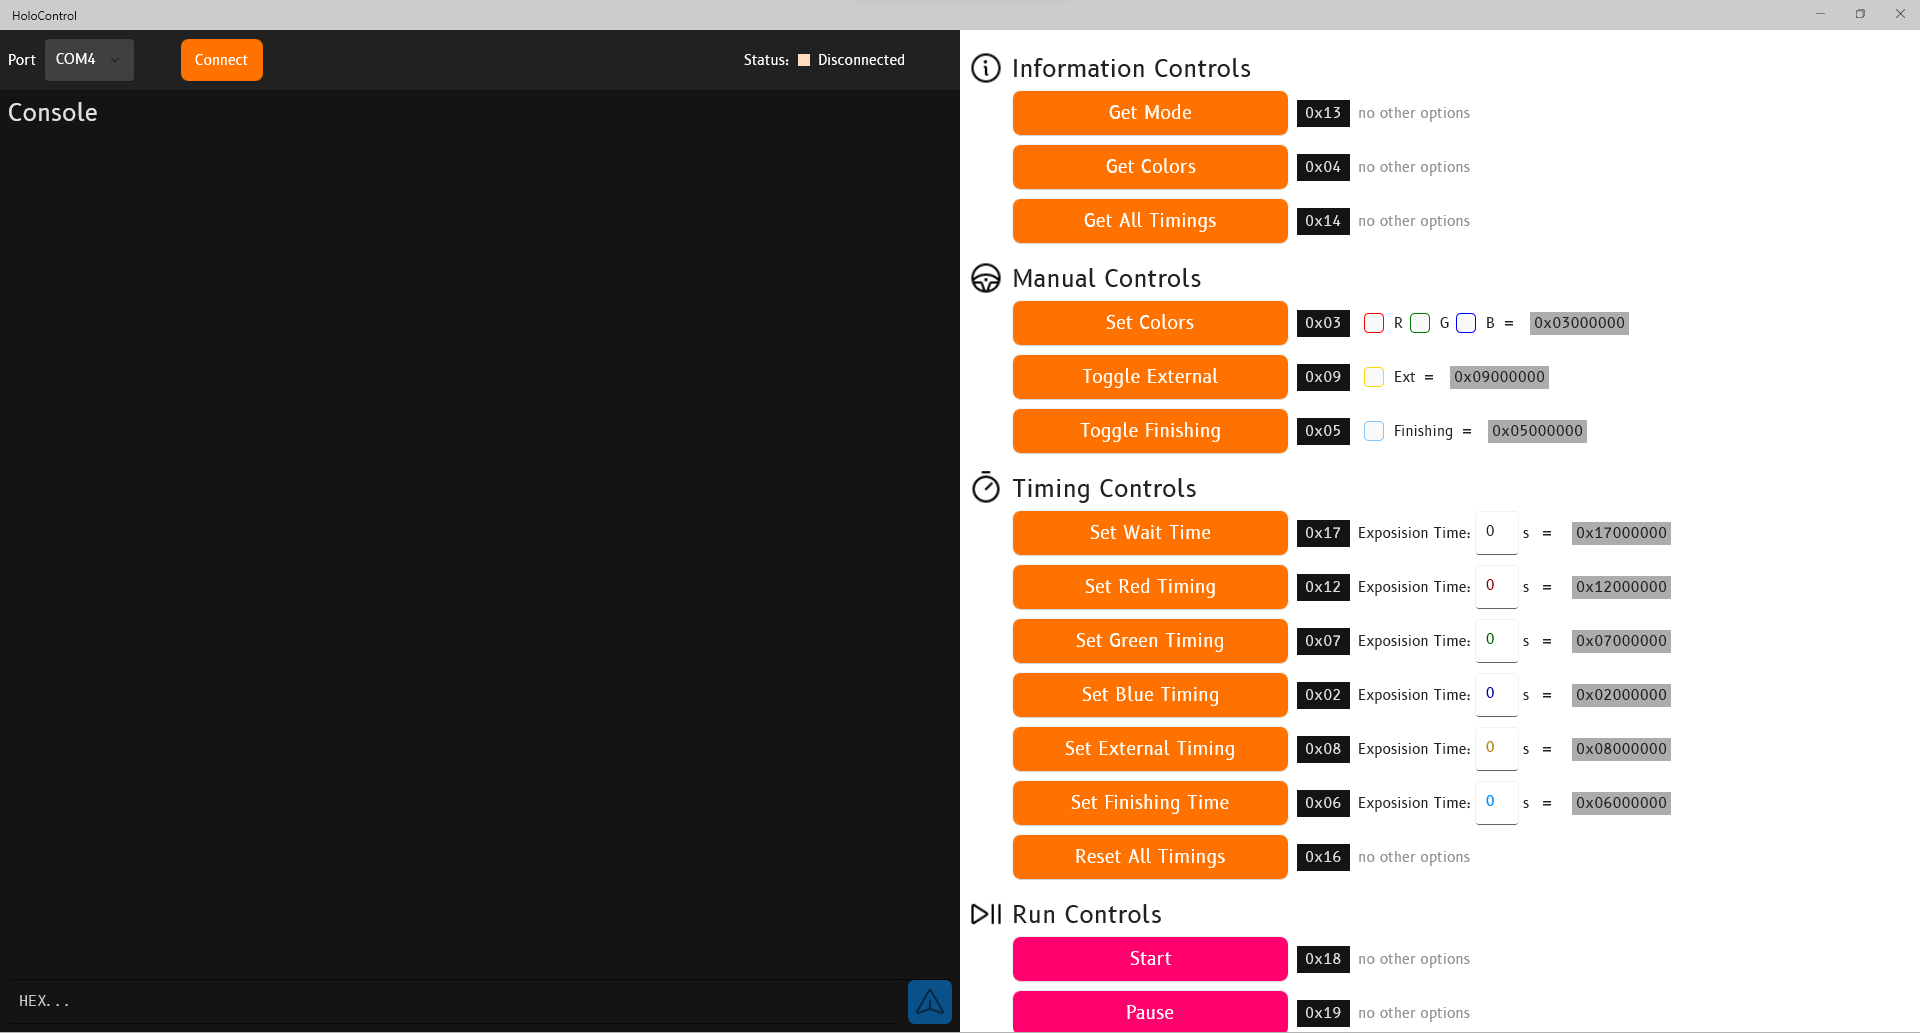
\includegraphics[width=\linewidth]{../img/HoloControl-UI.png}
    \caption{Snímek obrazovky standardního režimu aplikace \textbf{HoloControl}}
    \label{img:holocontrol}
\end{figure}

Obrázek \ref{img:holocontrol} ukazuje rozložení standardního režimu grafické aplikace. Levá strana slouží jako prostý terminál, kde v horní části lze ze seznamu připojených sériových portů zvolit ten, ke kterému je mikrokontroler připojený, a připojit se k němu. Dolní část je příkazový řádek, kam se vkládají instrukce v šestnáctkovém zápisu, a uprostřed se nachází záznam veškeré komunikace mezi aplikací a mikrokontrolerem.

Pravá strana pak obsahuje tlačítka pro vložení jednotlivých instrukcí a u instrukcí s argumenty také pole pro nastavení těchto argumentů. Uživatel při používání nastaví argumenty požadované instrukce a klikne na tlačítko této instrukce. Tím se instrukce s argumenty přeloženými do šestnáctkového zápisu vloží do příkazové řádky. Takto může uživatel zadat i několik instrukcí před tím, než je pomocí tlačítka vedle příkazové řádky odešle. Odeslané instrukce i odpověď mikrokontroleru se objeví v záznamu.

\medskip

Aplikace \textbf{HoloControl} byla naprogramována pomocí \textbf{.NET Multi-platform App UI} (\textbf{MAUI}), která umožňuje nasazení stejné aplikace pro systémy Windows, macOS, Android, iOS a Tizen \cite{maui}. Z těchto bylo z dispozičních důvodů využito pouze systémů Windows a Android, což ale stále umožní ovládání z počítačů, laptopů, tabletů i mobilních telefonů.

Aplikaci samozřejmě lze ovládat i dotykem, je dále responzivní vůči velikosti obrazovky i preferovanému světlému/tmavému režimu a je lokalizována do češtiny a angličtiny.

\medskip

V budoucnosti je v plánu aplikaci rozšířit o kioskový režim, ve kterém se již uživatel s instrukcemi vůbec nesetká a veškeré ovládání bude konáno výhradně graficky. Standardní režim byl takto navržen proto, aby studenti mohli nahlédnout a vyzkoušeli si práci s šestnáctkovou soustavou a sériovým terminálem; kioskový režim pak poslouží pro předváděcí účely.


\vfill
\noindent
\textit{Kompletní softwarová dokumentace bude zpracována a společně se zdrojovými kódy bude předána pracovišti po formálním ukončení projektu.}
\chapter*{Závěr}
\addcontentsline{toc}{chapter}{Závěr}
V rámci projektu byla úspěšně přestavěna úloha holografie na moderní barevné holografické desky \textbf{LitiHolo}. Při stavbě nového experimentálního uspořádání jsme rovnou pracovali na sekundárním cíli sestavení experimentu v kompaktní a mobilní podobě - celé experimentální uspořádání je sestaveno na přenosné desce velikosti $30\,\text{cm}\times 60\,\text{cm}$. Úloha lze velmi jednoduše převádět mezi reflexním a transmisním uspořádáním a v reflexním uspořádání lze vytvářet hologramy v plné barvě, bylo tedy dosaženo cíle chromatické holografie.

Chromatická transmisní holografie je v principu též možná, ovšem vzhledem nízkému světelnému výkonu použitých laserů by byly expoziční doby nepřijatelně dlouhé, jak z hlediska času studentů a vyučujících, tak kvůli vibracím, které při delších dobách expozice značně zhoršují kvalitu hologramu. Pro účely transmisní holografie lze do experimentálního uspořádání navést výkonný externí laser, pomocí kterého bude možné vytvořit alespoň monochromatické transmisní hologramy.

K optické části je v této zprávě také uvedeno několik potenciálních zlepšení, které spadají mimo rozsah a možnosti tohoto projektu. Ty poslouží pracovišti jako náměty na příležitostné zlepšení v budoucnu.

\medskip

Všechny lasery (tři barevné interní lasery a případný laser externí) jsou řízené plně elektronicky, a to včetně časování. K experimentu byl vytvořen elektronický obvod řízený mikrokontrolerem, který slouží primárně k přesnému odměření doby expozice jednotlivými barvami laserů. Díky tomu nejsou potřeba zásahy uživatele v průběhu expozice a rizika poškození hologramu, optických prvků, či zranění. Dále byla do uspořádání přidána bílá LED s vysokým světelným tokem pro dosvětlování holografických desek po expozici pro zvýšení kontrastu.

Ovládání mikrokontroleru je možné buďto v omezené míře pomocí fyzických tlačítek a přepínačů, nebo pomocí sériové komunikace. Tu lze realizovat buďto přímo skrze sériový terminál za použití přiložené instrukční sady, nebo pohodlněji pomocí grafické aplikace, která byla k tomuto projektu také vytvořena.

\medskip

Studijní text k úloze po domluvě s vedoucí projektu nebyl v rámci projektu přepracováván, nicméně i po formálním ukončení projektu budeme na přípravě úlohy pracovat dále a zlepšovat některé její aspekty, jako např. vytvoření kioskového režimu grafické aplikace, finalizace elektronického obvodu a vymodelování a výroba krytu na elektroniku, které vzhledem k časové vytíženosti nejsou krátkodobě realizovatelné.

Až po formálním dokončení projektu a finalizaci relevantních částí budou také zpracovány a pracovišti předány technické dokumentace jak k elektronické části, tak softwarové. Též bude předán zdrojový kód, který je k dispozici volně v repozitáři \url{https://github.com/Akimayo/HoloControl}. Technické dokumentace poslouží pro dlouhodobou udržitelnost experimentálního uspořádání, aby v budoucnu bylo možné provádět opravy či modifikace tohoto uspořádání.

\medskip

Primárního cíle projektu, chromatické holografie, bylo tedy dosaženo úspěšně. Společně s tím byl původní záměr doplněn o řadu provozních a technických rozšíření, která dělají experimentálnější uspořádání pohodlnější jak pro účely praktika, tak pro propagační akce a i pro běžný provoz v laboratoři. Nový studijní text k úloze nakonec v rámci projektu zpracován nebyl, nicméně bude vytvořen vedoucí úlohy a případně rozšířen o interaktivní prvky a simulace, které byly zmíněny jako jeden ze sekundárních cílů.

\medskip

Osobně mi projekt přinesl řadu praktických zkušeností v oblasti optiky a patřičný úžas nad kouzlem hologramů. Dále jsem měl mnoho prostoru na využití svých dovedností v oblasti elektroniky a programování, což vedlo na podstatné rozšíření původního záměru, díky kterému ale doufám bude experimentální uspořádání o to kvalitnější a zážitek studentů v praktiku OOEI lepší. Rozsáhlá práce na elektronické části taky přinesla řadu nových zkušeností a poučení do budoucna.

\printbibliography[title=Reference]

\appendix
\chapter{Protokol pro sériovou komunikaci s mikrokontrolerem\label{cpt:appendix}}
Pro rychlou referenci přikládáme do zprávy tabulku příkazů pro sériovou komunikaci s mikrokontrolerem.

\medskip

Mikrokontroler reaguje na čtyřbajtové instrukce, kde první bajt udává příkaz a zbylé tři bajty buďto jsou nevyužité, nesou stav zapnutí/vypnutí, nebo nesou počet milisekund. Z prvního bajtu jsou navíc příkazy vybírány pouze podle posledních čtyř bitů, což v kombinaci se zvolenými instrukčními kódy umožňuje jako první bit použít písmeno latinské abecedy. Instrukční kódy jsou zvoleny tak, aby bylo z písmene (prvního bajtu) jednoduše identifikovat příkaz.

V tabulce \ref{tbl:instrukce} jsou uvedeny všechny užitečné instrukce. Jelikož je nejvýhodnější příkazy zadávat pomocí zápisů/čísel v šestnáctkové soustavě, jsou instrukční kódy uváděny též v šestnáctkové soustavě (vypsány jsou vždy pouze kódy reprezentované posledními čtyřmi bity, na ASCII kód písmene lze šestnáctkový zápis převést přičtením $64_{10}=\mathtt{0x40}$). U příkazů, které jako argument přijímají čas v milisekundách, je nutné převést počet milisekund též do šestnáctkové soustavy.

\begin{table}[hp]
    \begin{adjustwidth}{-6em}{-3em}
        \caption{Instrukce pro sériovou komunikaci s mikrokontrolerem}
        \centering
        \begin{tabular}{|l|c|c|l|}
            \hline
            \textbf{Instruction} & \textbf{Code} & \textbf{Hex}           & \textbf{Parameter}                                        \\
            \hline
            Start                & \texttt{"x"}  & $\mathtt{0{\times}18}$ & \textit{none}                                             \\
            Pause                & \texttt{"y"}  & $\mathtt{0{\times}19}$ & \textit{none}                                             \\
            Stop                 & \texttt{"z"}  & $\mathtt{0{\times}1A}$ & \textit{none}                                             \\
            Set colors           & \texttt{"c"}  & $\mathtt{0{\times}03}$ & Every non-zero byte turns on its corresponding LED (RGB)  \\
            Set external         & \texttt{"i"}  & $\mathtt{0{\times}09}$ & Non-zero value turns on external laser                    \\
            Get colors           & \texttt{"d"}  & $\mathtt{0{\times}04}$ & \textit{none}                                             \\
            Toggle white         & \texttt{"e"}  & $\mathtt{0{\times}05}$ & Non-zero value turns on finishing white LED               \\
            Get mode             & \texttt{"s"}  & $\mathtt{0{\times}13}$ & \textit{none}                                             \\
            Buzz                 & \texttt{"u"}  & $\mathtt{0{\times}15}$ & 3-byte time to buzz for in milliseconds                   \\
            Set red time         & \texttt{"r"}  & $\mathtt{0{\times}12}$ & 3-byte time of red laser in milliseconds                  \\
            Set green time       & \texttt{"g"}  & $\mathtt{0{\times}07}$ & 3-byte time of green laser in milliseconds                \\
            Set blue time        & \texttt{"b"}  & $\mathtt{0{\times}02}$ & 3-byte time of blue laser in milliseconds                 \\
            Set external time    & \texttt{"h"}  & $\mathtt{0{\times}08}$ & 3-byte time of external laser in milliseconds             \\
            Set finishing time   & \texttt{"f"}  & $\mathtt{0{\times}06}$ & 3-byte time of white light in milliseconds after exposing \\
            Set wait time        & \texttt{"w"}  & $\mathtt{0{\times}17}$ & 3-byte time of waiting before exposing                    \\
            Show all times       & \texttt{"t"}  & $\mathtt{0{\times}14}$ & \textit{none}                                             \\
            Reset all times      & \texttt{"v"}  & $\mathtt{0{\times}16}$ & \textit{none}                                             \\
            \hline
        \end{tabular}
    \end{adjustwidth}
    \label{tbl:instrukce}
\end{table}
\end{document}